% !TeX spellcheck = hu_HU
% !TeX encoding = UTF-8
% !TeX program = xelatex
% TODO Change language to en_GB (recommended) or en_US for English documents
\documentclass[11pt,a4paper,oneside]{report}             % Single-side
%\documentclass[11pt,a4paper,twoside,openright]{report}  % Duplex

% thanks to http://tex.stackexchange.com/a/47579/71109
\usepackage{ifxetex}
\usepackage{ifluatex}
\newif\ifxetexorluatex % a new conditional starts as false
\ifnum 0\ifxetex 1\fi\ifluatex 1\fi>0
   \xetexorluatextrue
\fi

\ifxetexorluatex
  \usepackage{fontspec}
\else
  \usepackage[T1]{fontenc}
  \usepackage[utf8]{inputenc}
  \usepackage[lighttt]{lmodern}
\fi

\usepackage[english,magyar]{babel} % Alapértelmezés szerint utoljára definiált nyelv lesz aktív, de később külön beállítjuk az aktív nyelvet.

%\usepackage{cmap}
\usepackage{amsfonts,amsmath,amssymb} % Mathematical symbols.
%\usepackage[ruled,boxed,resetcount,linesnumbered]{algorithm2e} % For pseudocodes. % beware: this is not compatible with LuaLaTeX, see http://tex.stackexchange.com/questions/34814/lualatex-and-algorithm2e
\usepackage{booktabs} % For publication quality tables for LaTeX
\usepackage{graphicx}

%\usepackage{fancyhdr}
%\usepackage{lastpage}

\usepackage{anysize}
%\usepackage{sectsty}
\usepackage{setspace} % For setting line spacing

\usepackage[unicode]{hyperref} % For hyperlinks in the generated document.
\usepackage{xcolor}
\usepackage{listings} % For source code snippets.

\usepackage[amsmath,thmmarks]{ntheorem} % Theorem-like environments.

\usepackage[hang]{caption}

\singlespacing

\newcommand{\selecthungarian}{
	\selectlanguage{magyar}
	\setlength{\parindent}{2em}
	\setlength{\parskip}{0em}
	\frenchspacing
}

\newcommand{\selectenglish}{
	\selectlanguage{english}
	\setlength{\parindent}{0em}
	\setlength{\parskip}{0.5em}
	\nonfrenchspacing
	\renewcommand{\figureautorefname}{Figure}
	\renewcommand{\tableautorefname}{Table}
	\renewcommand{\partautorefname}{Part}
	\renewcommand{\chapterautorefname}{Chapter}
	\renewcommand{\sectionautorefname}{Section}
	\renewcommand{\subsectionautorefname}{Section}
	\renewcommand{\subsubsectionautorefname}{Section}
}

\usepackage[numbers]{natbib}
\usepackage{xspace}
\usepackage{todonotes}

%TODO Set the main variables
\newcommand{\vikszerzoVezeteknev}{Bekő}
\newcommand{\vikszerzoKeresztnev}{Mária}

\newcommand{\vikkonzulensAMegszolitas}{}
\newcommand{\vikkonzulensAVezeteknev}{Semeráth}
\newcommand{\vikkonzulensAKeresztnev}{Oszkár}

\newcommand{\vikkonzulensBMegszolitas}{}
\newcommand{\vikkonzulensBVezeteknev}{}
\newcommand{\vikkonzulensBKeresztnev}{}

\newcommand{\vikkonzulensCMegszolitas}{}
\newcommand{\vikkonzulensCVezeteknev}{}
\newcommand{\vikkonzulensCKeresztnev}{}

\newcommand{\vikcim}{Gráfmintaillesztő rendszerek tesztelése automatikus gráfgenerátorokkal} % Cím
\newcommand{\viktanszek}{\bmemit} % Tanszék
\newcommand{\vikdoktipus}{\bsc} % Dokumentum típusa (\bsc vagy \msc)
\newcommand{\vikmunkatipusat}{TDK dolgozat} % a "hallgató nyilatkozat" részhez: szakdolgozatot vagy diplomatervet

%--------------------------------------------------------------------------------------
% TDK-specifikus változók
%--------------------------------------------------------------------------------------
\newcommand{\tdkszerzoB}{} % Második szerző neve; hagyd üresen, ha egyedül írtad a TDK-t.
\newcommand{\tdkev}{2018} % A dolgozat írásának éve (pl. "2014") (Ez OTDK-nál eltérhet az aktuális évtől.)

% További adatok az OTDK címlaphoz (BME-s TDK-hoz nem kell kitölteni)
\newcommand{\tdkevfolyamA}{V} % Első szerző évfolyama, római számmal (pl. IV).
\newcommand{\tdkevfolyamB}{} % Második szerző évfolyama, római számmal (pl. III).
\newcommand{\tdkkonzulensbeosztasA}{doktorandusz} % Első konzulens beosztása (pl. egyetemi docens)
\newcommand{\tdkkonzulensbeosztasB}{} % Második konzulens beosztása (pl. egyetemi docens)

\definecolor{backgroundColor}{rgb}{0.89,0.92,0.95}
\definecolor{darkerbackgroundColor}{rgb}{0.623,0.644,0.664}

\definecolor{keywordcolor}{rgb}{0.5,0,0.1}
\definecolor{commentcolor}{rgb}{0,0.3,0.1}
\definecolor{stringcolor}{rgb}{0,0,1}
\definecolor{emphColor}{rgb}{0,0.1,0.49}

\lstdefinelanguage{viatra}
{morekeywords={@QueryBasedFeature,@Constraint,count,pattern,package,
		neg,find,import,true,false,or,check,job,action,state,severity,location,message,
		oclIsKindOf,self,exists,includes,invariant,class,private},
	emph={openCypher,Cypher,QueryOptions,statement,QueryOptions,CypherOption,versionNumber,configurationOption,VersionNumber,versionNumber,ConfigurationOption,key,value,Statement,Query,RegularQuery,BulkImportQuery,periodicCommitHint,loadCSVQuery,PeriodicCommitHint,numberOfRowsPerCommit,LoadCSVQuery,loadCSV,singleQuery,Union,all,singleQuery,SingleQuery,SinglePartQuery,readingClauses,return,updatingClauses,MultiPartQuery,subQueries,singlePartQuery,MultiPartSubQuery,readingClauses,updatingClauses,withPart,Clause,UpdatingClause,ReadingClause,Command,CreateUniqueConstraint,CreateNodePropertyExistenceConstraint,CreateRelationshipPropertyExistenceConstraint,CreateIndex,index,DropUniqueConstraint,uniqueConstraint,DropNodePropertyExistenceConstraint,nodePropertyExistenceConstraint,DropRelationshipPropertyExistenceConstraint,relationshipPropertyExistenceConstraint,DropIndex,index,Index,nodeLabel,propertyKeyName,UniqueConstraint,variable,nodeLabel,propertyExpression,NodePropertyExistenceConstraint,variable,nodeLabel,propertyExpression,RelationshipPropertyExistenceConstraint,relationshipPattern,propertyExpression,RelationshipPatternSyntax,incoming,variable,relType,outgoing,LoadCSV,withHeaders,expression,variable,fieldterminator,Match,optional,pattern,hints,where,Unwind,expression,variable,Merge,patternPart,mergeActions,MergeAction,action,set,Create,uniqueContraint,pattern,Set,setItems,SetItem,propertyExpression,expression,variable,Delete,detach,expressions,Remove,removeItems,RemoveItem,Foreach,variable,expression,updatingClauses,InQueryCall,invocation,yieldItems,StandaloneCall,invocation,yieldItems,YieldItems,items,YieldItem,field,variable,With,distint,returnBody,where,Return,return,distinct,body,ReturnBody,returnItems,order,skip,limit,ReturnItems,all,items,ReturnItem,expression,alias,Order,orderBy,Skip,skip,Limit,limit,SortItem,expression,sort,Hint,Start,startPoint,where,StartPoint,variable,lookup,Lookup,NodeLookup,RelationshipLookup,IdentifiedIndexLookup,indexName,key,value,legacyParameter,IndexQuery,indexName,query,parameter,IdLookup,ids,legacyParameter,wildcard,LiteralIds,ids,Where,expression,Pattern,patterns,PatternPart,var,part,AnonymousPatternPart,ShortestPathPattern,patternElement,PatternElement,nodepattern,chain,NodePattern,variable,properties,PatternElementChain,relationshipPattern,nodePattern,RelationshipPattern,incoming,detail,outgoing,RelationshipDetail,variable,optional,range,properties,Properties,RelationshipTypes,relTypeNames,NodeLabels,nodeLabels,NodeLabel,labelName,RangeLiteral,lower,variableLength,upper,Expression,propertyLookups,Literal,BooleanLiteral,value,ListLiteral,expressions,Reduce,accumulator,accumulatorExpression,idInColl,expression,ParenthesizedExpression,expression,RelationshipsPattern,nodePattern,chain,FilterExpression,idInColl,where,IdInColl,variable,expression,FunctionInvocation,functionName,distinct,parameter,ExplicitProcedureInvocation,procedureName,parameter,ImplicitProcedureInvocation,procedureName,ProcedureName,namespace,name,ListComprehension,filterExpression,expression,PatternComprehension,pathVariable,pattern,where,expression,PropertyLookup,propertyKeyName,propertyOperator,CaseExpression,caseAlternatives,caseExpression,elseExpression,CaseAlternatives,when,then,VariableDeclaration,name,StringLiteral,value,NumberLiteral,value,MapLiteral,entries,MapLiteralEntry,key,value,LegacyParameter,parameter,Parameter,parameter,PropertyExpression,DecimalInteger,value,AllOptions,explain,profile,cypherOption,CombinedQuery,singleQuery,union,RemoveItemLabel,variable,RemoveItemProperty,propertyExpression,IndexHint,variable,nodeLabel,propertyKeyName,JoinHint,variables,ScanHint,variable,nodeLabel,ShortestPath,AllShortestPaths,OrExpression,left,operator,right,XorExpression,left,operator,right,AndExpression,left,operator,right,NotExpressionoperator,left,ComparisonExpression,left,operator,right,AddOrSubtractExpression,left,operator,right,MultiplyDivideModuloExpression,left,operator,right,PowerOfExpression,left,operator,right,UnaryAddOrSubtractExpression,operator,left,IndexLookupExpression,left,expression,IndexRangeExpression,left,lower,upper,RegExpMatchingExpression,left,right,InCollectionExpression,left,right,StartsWithExpression,left,right,EndsWithExpression,left,right,ContainsExpression,left,right,IsNullExpression,left,IsNotNullExpression,left,PropertyLookupExpression,left,NodeLabelsExpression,left,Count,Filter,filterExpression,Extract,filterExpression,expression,All,filterExpression,Any,filterExpression,None,filterExpression,Single,filterExpression,VariableRef,variableRef,NULL},
	emphstyle={\color{emphColor}},
	sensitive=true, morecomment=[l]{//}, morecomment=[s]{/*}{*/},
	morestring=[b]{"}
}
\lstdefinestyle{viatrasmall}{
	basicstyle=\scriptsize\ttfamily,
	commentstyle=\color{commentcolor}\ttfamily,
	stringstyle=\color{stringcolor}\ttfamily,
	%frameround=tttt,
	captionpos=b,
	keywordstyle=\color{keywordcolor}\bfseries\ttfamily,
	showstringspaces=false,
	tabsize=2,
	language=viatra,
	escapeinside={(*@}{@*)},
	breaklines=false
}
\lstdefinestyle{viatrabig}{
	basicstyle=\ttfamily,
	commentstyle=\color{commentcolor}\ttfamily,
	stringstyle=\color{stringcolor}\ttfamily,
	%frameround=tttt,
	captionpos=b,
	keywordstyle=\color{keywordcolor}\bfseries\ttfamily,
	showstringspaces=false,
	tabsize=2,
	language=viatra,
	escapeinside={(*@}{@*)},
	breaklines=false
}
\newcommand{\viatraStyle}[1]{\lstinline[style=viatrabig]@#1@}
\newcommand{\mm}[1]{{\color{emphColor}\textsf{#1}}}
\newcommand{\szerzoMeta}{\vikszerzoVezeteknev{} \vikszerzoKeresztnev} % egy szerző esetén
%\newcommand{\szerzoMeta}{\vikszerzoVezeteknev{} \vikszerzoKeresztnev, \tdkszerzoB} % két szerző esetén

%TODO Language configuration -- choose one
% Beállítások magyar nyelvű dolgozathoz
%--------------------------------------------------------------------------------------
% Elnevezések
%--------------------------------------------------------------------------------------
\newcommand{\bme}{Budapesti Műszaki és Gazdaságtudományi Egyetem}
\newcommand{\vik}{Villamosmérnöki és Informatikai Kar}

\newcommand{\bmemit}{Méréstechnika és Információs Rendszerek Tanszék}

\newcommand{\keszitette}{Készítette}
\newcommand{\konzulens}{Konzulens}

\newcommand{\bsc}{Szakdolgozat}
\newcommand{\msc}{Diplomaterv}
\newcommand{\tdk}{TDK dolgozat}
\newcommand{\bsconlab}{BSc Önálló laboratórium}
\newcommand{\msconlabi}{MSc Önálló laboratórium 1.}
\newcommand{\msconlabii}{MSc Önálló laboratórium 2.}

\newcommand{\pelda}{Példa}
\newcommand{\definicio}{Definíció}
\newcommand{\tetel}{Tétel}

\newcommand{\bevezetes}{Bevezetés}
\newcommand{\koszonetnyilvanitas}{Köszönetnyilvánítás}
\newcommand{\fuggelek}{Függelék}

\newcommand{\eloismeretek}{Előismeretek}
\newcommand{\osszefoglalas}{Összefoglalás}
\newcommand{\attekintes}{Áttekintés}
\newcommand{\ellaboration}{Mi ennek a magyar neve}
\newcommand{\evaluation}{Értékelés}


% Opcionálisan átnevezhető címek
%\addto\captionsmagyar{%
%\renewcommand{\listfigurename}{Saját ábrajegyzék cím}
%\renewcommand{\listtablename}{Saját táblázatjegyzék cím}
%\renewcommand{\bibname}{Saját irodalomjegyzék név}
%}

\newcommand{\szerzo}{\vikszerzoVezeteknev{} \vikszerzoKeresztnev}
\newcommand{\vikkonzulensA}{\vikkonzulensAMegszolitas\vikkonzulensAVezeteknev{} \vikkonzulensAKeresztnev}
\newcommand{\vikkonzulensB}{\vikkonzulensBMegszolitas\vikkonzulensBVezeteknev{} \vikkonzulensBKeresztnev}
\newcommand{\vikkonzulensC}{\vikkonzulensCMegszolitas\vikkonzulensCVezeteknev{} \vikkonzulensCKeresztnev}

\newcommand{\selectthesislanguage}{\selecthungarian}

\bibliographystyle{huplain}

\def\lstlistingname{lista}

\newcommand{\appendixnumber}{6}  % a fofejezet-szamlalo az angol ABC 6. betuje (F) lesz

% Settings for English documents
%%--------------------------------------------------------------------------------------
% Elnevezések
%--------------------------------------------------------------------------------------
\newcommand{\bme}{Budapest University of Technology and Economics}
\newcommand{\vik}{Faculty of Electrical Engineering and Informatics}

\newcommand{\bmemit}{Department of Measurement and Information Systems}

\newcommand{\keszitette}{Author}
\newcommand{\konzulens}{Advisor}

\newcommand{\bsc}{Bachelor's Thesis}
\newcommand{\msc}{Master's Thesis}
\newcommand{\tdk}{Scientific Students' Association Report}
\newcommand{\bsconlab}{BSc Project Laboratory}
\newcommand{\msconlabi}{MSc Project Laboratory 1}
\newcommand{\msconlabii}{MSc Project Laboratory 2}

\newcommand{\pelda}{Example}
\newcommand{\definicio}{Definition}
\newcommand{\tetel}{Theorem}

\newcommand{\bevezetes}{Introduction}
\newcommand{\koszonetnyilvanitas}{Acknowledgements}
\newcommand{\fuggelek}{Appendix}

% Optional custom titles
%\addto\captionsenglish{%
%\renewcommand*{\listfigurename}{Your list of figures title}
%\renewcommand*{\listtablename}{Your list of tables title}
%\renewcommand*{\bibname}{Your bibliography title}
%}

\newcommand{\szerzo}{\vikszerzoKeresztnev{} \vikszerzoVezeteknev}
\newcommand{\vikkonzulensA}{\vikkonzulensAMegszolitas\vikkonzulensAKeresztnev{} \vikkonzulensAVezeteknev}
\newcommand{\vikkonzulensB}{\vikkonzulensBMegszolitas\vikkonzulensBKeresztnev{} \vikkonzulensBVezeteknev}
\newcommand{\vikkonzulensC}{\vikkonzulensCMegszolitas\vikkonzulensCKeresztnev{} \vikkonzulensCVezeteknev}

\newcommand{\selectthesislanguage}{\selectenglish}

\bibliographystyle{plainnat}

\newcommand{\ie}{i.e.\@\xspace}
\newcommand{\Ie}{I.e.\@\xspace}
\newcommand{\eg}{e.g.\@\xspace}
\newcommand{\Eg}{E.g.\@\xspace}
\newcommand{\etal}{et al.\@\xspace}
\newcommand{\etc}{etc.\@\xspace}
\newcommand{\vs}{vs.\@\xspace}
\newcommand{\viz}{viz.\@\xspace} % videlicet
\newcommand{\cf}{cf.\@\xspace} % confer
\newcommand{\Cf}{Cf.\@\xspace}
\newcommand{\wrt}{w.r.t.\@\xspace} % with respect to
\newcommand{\approximately}{approx.\xspace}

\newcommand{\appendixnumber}{1}  % a fofejezet-szamlalo az angol ABC 1. betuje (A) lesz


%--------------------------------------------------------------------------------------
% Page layout setup
%--------------------------------------------------------------------------------------
% we need to redefine the pagestyle plain
% another possibility is to use the body of this command without \fancypagestyle
% and use \pagestyle{fancy} but in that case the special pages
% (like the ToC, the References, and the Chapter pages)remain in plane style

\pagestyle{plain}
\marginsize{35mm}{25mm}{15mm}{15mm}

\setcounter{tocdepth}{3}
%\sectionfont{\large\upshape\bfseries}
\setcounter{secnumdepth}{3}

\sloppy % Margón túllógó sorok tiltása.
\widowpenalty=10000 \clubpenalty=10000 %A fattyú- és árvasorok elkerülése
\def\hyph{-\penalty0\hskip0pt\relax} % Kötőjeles szavak elválasztásának engedélyezése


%--------------------------------------------------------------------------------------
% Setup hyperref package
%--------------------------------------------------------------------------------------
\hypersetup{
    % bookmarks=true,            % show bookmarks bar?
    unicode=true,              % non-Latin characters in Acrobat's bookmarks
    pdftitle={\vikcim},        % title
    pdfauthor={\szerzoMeta},    % author
    pdfsubject={\vikdoktipus}, % subject of the document
    pdfcreator={\szerzoMeta},   % creator of the document
    pdfproducer={},    % producer of the document
    pdfkeywords={},    % list of keywords (separate then by comma)
    pdfnewwindow=true,         % links in new window
    colorlinks=true,           % false: boxed links; true: colored links
    linkcolor=black,           % color of internal links
    citecolor=black,           % color of links to bibliography
    filecolor=black,           % color of file links
    urlcolor=black             % color of external links
}


%--------------------------------------------------------------------------------------
% Set up listings
%--------------------------------------------------------------------------------------
\definecolor{lightgray}{rgb}{0.95,0.95,0.95}
\lstset{
	basicstyle=\scriptsize\ttfamily, % print whole listing small
	keywordstyle=\color{black}\bfseries, % bold black keywords
	identifierstyle=, % nothing happens
	% default behavior: comments in italic, to change use
	% commentstyle=\color{green}, % for e.g. green comments
	stringstyle=\scriptsize,
	showstringspaces=false, % no special string spaces
	aboveskip=3pt,
	belowskip=3pt,
	backgroundcolor=\color{lightgray},
	columns=flexible,
	keepspaces=true,
	escapeinside={(*@}{@*)},
	captionpos=b,
	breaklines=true,
	frame=single,
	float=!ht,
	tabsize=2,
	literate=*
		{á}{{\'a}}1	{é}{{\'e}}1	{í}{{\'i}}1	{ó}{{\'o}}1	{ö}{{\"o}}1	{ő}{{\H{o}}}1	{ú}{{\'u}}1	{ü}{{\"u}}1	{ű}{{\H{u}}}1
		{Á}{{\'A}}1	{É}{{\'E}}1	{Í}{{\'I}}1	{Ó}{{\'O}}1	{Ö}{{\"O}}1	{Ő}{{\H{O}}}1	{Ú}{{\'U}}1	{Ü}{{\"U}}1	{Ű}{{\H{U}}}1
}


%--------------------------------------------------------------------------------------
% Set up theorem-like environments
%--------------------------------------------------------------------------------------
% Using ntheorem package -- see http://www.math.washington.edu/tex-archive/macros/latex/contrib/ntheorem/ntheorem.pdf

\theoremstyle{plain}
\theoremseparator{.}
\newtheorem{example}{\pelda}

\theoremseparator{.}
%\theoremprework{\bigskip\hrule\medskip}
%\theorempostwork{\hrule\bigskip}
\theorembodyfont{\upshape}
\theoremsymbol{{\large \ensuremath{\centerdot}}}
\newtheorem{definition}{\definicio}

\theoremseparator{.}
%\theoremprework{\bigskip\hrule\medskip}
%\theorempostwork{\hrule\bigskip}
\newtheorem{theorem}{\tetel}


%--------------------------------------------------------------------------------------
% Some new commands and declarations
%--------------------------------------------------------------------------------------
\newcommand{\code}[1]{{\upshape\ttfamily\scriptsize\indent #1}}
\newcommand{\doi}[1]{DOI: \href{http://dx.doi.org/\detokenize{#1}}{\raggedright{\texttt{\detokenize{#1}}}}} % A hivatkozások közt így könnyebb DOI-t megadni.

\DeclareMathOperator*{\argmax}{arg\,max}
%\DeclareMathOperator*[1]{\floor}{arg\,max}
\DeclareMathOperator{\sign}{sgn}
\DeclareMathOperator{\rot}{rot}


%--------------------------------------------------------------------------------------
% Setup captions
%--------------------------------------------------------------------------------------
\captionsetup[figure]{
	width=.75\textwidth,
	aboveskip=10pt}

\renewcommand{\captionlabelfont}{\bf}
%\renewcommand{\captionfont}{\footnotesize\it}

%--------------------------------------------------------------------------------------
% Hyphenation exceptions
%--------------------------------------------------------------------------------------
\hyphenation{Shakes-peare Mar-seilles ár-víz-tű-rő tü-kör-fú-ró-gép}


\author{\vikszerzo}
\title{\viktitle}

%--------------------------------------------------------------------------------------
% Table of contents and the main text
%--------------------------------------------------------------------------------------
\begin{document}

%TODO These define guidelines -- remove these
%~~~~~~~~~~~~~~~~~~~~~~~~~~~~~~~~~~~~~~~~~~~~~~~~~~~~~~~~~~~~~~~~~~~~~~~~~~~~~~~~~~~~~~
%\pagenumbering{gobble}
\selecthungarian
%--------------------------------------------------------------------------------------
% Rovid formai es tartalmi tajekoztato
%--------------------------------------------------------------------------------------

\footnotesize
\begin{center}
\large
\textbf{\Large Általános információk, a diplomaterv szerkezete}\\
\end{center}

A diplomaterv szerkezete a BME Villamosmérnöki és Informatikai Karán:
\begin{enumerate}
\item	Diplomaterv feladatkiírás
\item	Címoldal
\item	Tartalomjegyzék
\item	A diplomatervező nyilatkozata az önálló munkáról és az elektronikus adatok kezeléséről
\item	Tartalmi összefoglaló magyarul és angolul
\item	Bevezetés: a feladat értelmezése, a tervezés célja, a feladat indokoltsága, a diplomaterv felépítésének rövid összefoglalása
\item	A feladatkiírás pontosítása és részletes elemzése
\item	Előzmények (irodalomkutatás, hasonló alkotások), az ezekből levonható következtetések
\item	A tervezés részletes leírása, a döntési lehetőségek értékelése és a választott megoldások indoklása
\item	A megtervezett műszaki alkotás értékelése, kritikai elemzése, továbbfejlesztési lehetőségek
\item	Esetleges köszönetnyilvánítások
\item	Részletes és pontos irodalomjegyzék
\item	Függelék(ek)
\end{enumerate}

Felhasználható a következő oldaltól kezdődő \LaTeX diplomatervsablon dokumentum tartalma. 

A diplomaterv szabványos méretű A4-es lapokra kerüljön. Az oldalak tükörmargóval készüljenek (mindenhol 2,5~cm, baloldalon 1~cm-es kötéssel). Az alapértelmezett betűkészlet a 12 pontos Times New Roman, másfeles sorközzel, de ettől kismértékben el lehet térni, ill. más betűtípus használata is megengedett.

Minden oldalon -- az első négy szerkezeti elem kivételével -- szerepelnie kell az oldalszámnak.

A fejezeteket decimális beosztással kell ellátni. Az ábrákat a megfelelő helyre be kell illeszteni, fejezetenként decimális számmal és kifejező címmel kell ellátni. A fejezeteket decimális aláosztással számozzuk, maximálisan 3 aláosztás mélységben (pl. 2.3.4.1.). Az ábrákat, táblázatokat és képleteket célszerű fejezetenként külön számozni (pl. 2.4. ábra, 4.2. táblázat vagy képletnél (3.2)). A fejezetcímeket igazítsuk balra, a normál szövegnél viszont használjunk sorkiegyenlítést. Az ábrákat, táblázatokat és a hozzájuk tartozó címet igazítsuk középre. A cím a jelölt rész alatt helyezkedjen el.

A képeket lehetőleg rajzoló programmal készítsék el, az egyenleteket egyenlet-szerkesztő segítségével írják le (A \LaTeX~ehhez kézenfekvő megoldásokat nyújt).

Az irodalomjegyzék szövegközi hivatkozása történhet sorszámozva (ez a preferált megoldás) vagy a Harvard-rendszerben (a szerző és az évszám megadásával). A teljes lista névsor szerinti sorrendben a szöveg végén szerepeljen (sorszámozott irodalmi hivatkozások esetén hivatkozási sorrendben). A szakirodalmi források címeit azonban mindig az eredeti nyelven kell megadni, esetleg zárójelben a fordítással. A listában szereplő valamennyi publikációra hivatkozni kell a szövegben (a \LaTeX-sablon a Bib\TeX~segítségével mindezt automatikusan kezeli). Minden publikáció a szerzők után a következő adatok szerepelnek: folyóirat cikkeknél a pontos cím, a folyóirat címe, évfolyam, szám, oldalszám tól-ig. A folyóiratok címét csak akkor rövidítsük, ha azok nagyon közismertek vagy nagyon hosszúak. Internetes hivatkozások megadásakor fontos, hogy az elérési út előtt megadjuk az oldal tulajdonosát és tartalmát (mivel a link egy idő után akár elérhetetlenné is válhat), valamint az elérés időpontját.

\vspace{5mm}
Fontos:
\begin{itemize}
	\item A szakdolgozatkészítő / diplomatervező nyilatkozata (a jelen sablonban szereplő szövegtartalommal) kötelező előírás, Karunkon ennek hiányában a szakdolgozat/diplomaterv nem bírálható és nem védhető!
	\item Mind a dolgozat, mind a melléklet maximálisan 15~MB méretű lehet!
\end{itemize}

\vspace{5mm}
\begin{center}
Jó munkát, sikeres szakdolgozatkészítést, ill. diplomatervezést kívánunk!
\end{center}

\normalsize
\selectthesislanguage

%\textbf{}\pagenumbering{gobble}
%--------------------------------------------------------------------------------------
% Feladatkiiras (a tanszeken atveheto, kinyomtatott valtozat)
%--------------------------------------------------------------------------------------
\clearpage
\begin{center}
\large
\textbf{FELADATKIÍRÁS}\\
\end{center}

A feladatkiírást a tanszéki adminisztrációban lehet átvenni, és a leadott munkába eredeti, tanszéki pecséttel ellátott és a tanszékvezető által aláírt lapot kell belefűzni (ezen oldal \emph{helyett}, ez az oldal csak útmutatás). Az elektronikusan feltöltött dolgozatban már nem kell beleszerkeszteni ezt a feladatkiírást.


\selectthesislanguage

%TODO Titlepage -- choose one from below
%~~~~~~~~~~~~~~~~~~~~~~~~~~~~~~~~~~~~~~~~~~~~~~~~~~~~~~~~~~~~~~~~~~~~~~~~~~~~~~~~~~~~~~
%\hypersetup{pageanchor=false}
%--------------------------------------------------------------------------------------
%	The title page
%--------------------------------------------------------------------------------------
\begin{titlepage}
\begin{center}

\includegraphics[width=60mm,keepaspectratio]{figures/bme_logo.pdf}\\
\vspace{0.3cm}
\textbf{\bme}\\
\textmd{\vik}\\
\textmd{\viktanszek}\\[5cm]

\vspace{0.4cm}
{\huge \bfseries \vikcim}\\[0.8cm]
\vspace{0.5cm}
\textsc{\Large \vikdoktipus}\\[4cm]

{
	\renewcommand{\arraystretch}{0.85}
	\begin{tabular}{cc}
	 \makebox[7cm]{\emph{\keszitette}} & \makebox[7cm]{\emph{\konzulens}} \\ \noalign{\smallskip}
	 \makebox[7cm]{\szerzo} & \makebox[7cm]{\vikkonzulensA} \\
	  & \makebox[7cm]{\vikkonzulensB} \\
	  & \makebox[7cm]{\vikkonzulensC} \\
	\end{tabular}
}

\vfill
{\large \today}
\end{center}
\end{titlepage}
\hypersetup{pageanchor=false}

		   % Szakdolgozat/Diplomaterv címlap
%% TDK címlap
\begin{titlepage}
  \begin{center}  
  
\includegraphics[width=7cm]{./figures/bme_logo.pdf}
  \vspace{0.3cm}
  
  \bme \\
  \vik \\
  \viktanszek \\
  \vspace{5cm}
  
  \huge {\vikcim}
  \vspace{1.5cm}
  
  \large {\textbf{\tdk}}
  \vfill
    
  {\Large 
  	\keszitette: \\ \vspace{0.3cm}
  	\szerzo \\
%	\tdkszerzoB \\
  	\vspace{1.5cm}
  	\konzulens: \\ \vspace{0.3cm}
  	\vikkonzulensA \\
%	\vikkonzulensB \\
  }
  
  \vspace{2cm}
  \large {\tdkev}
 \end{center}
\end{titlepage}
%% Címlap vége
	% TDK címlap
%%% OTDK külső címlap
\begin{titlepage}
  	$\;$ 
	\vspace{5cm}
	
	\begin{center}
	\Huge
	\textbf{TDK-dolgozat}\let\thefootnote\relax\footnote{A dolgozat bemutatását a XXXXXXXXX  ``Lorem ipsum dolor sit amet'' című program támogatta.}
	\end{center}
	
	\vspace{13cm}
	
	\Large
	\hspace{8cm} \szerzo
	
	\hspace{8cm} \tdkszerzoB
	
	\hspace{8cm} \tdkev.
\end{titlepage}

\newpage
\thispagestyle{empty}


%% OTDK belső címlap
\begin{titlepage}
  \begin{center}  
  
\includegraphics[width=7cm]{./figures/bme_logo.pdf}
  \vspace{0.3cm}
  
  \bme \\
  \vik \\
  \viktanszek \\
  \vspace{3.5cm}
  
  \huge {\vikcim}
  \vspace{1.5cm}
  
  \large {\textbf{\vikdoktipus}}
  \vfill
    
  {\Large 
  	{\large \keszitette:} \\ \vspace{0.2cm}
  	\szerzo \\ \tdkevfolyamA. évfolyam \\
	\vspace{0.5cm}
	\tdkszerzoB \\ \tdkevfolyamB. évfolyam \\
  	\vspace{1.5cm}
  	{\large \konzulens:} \\ \vspace{0.2cm}
  	\vikkonzulensA,\\ \tdkkonzulensbeosztasA \\
  	\vspace{0.5cm}
  	\vikkonzulensB,\\ \tdkkonzulensbeosztasB \\
  }
  
  \vspace{2cm}
  \large {\tdkev.}
  
 \end{center}
\end{titlepage}   % OTDK címlap


% Table of Contents
%~~~~~~~~~~~~~~~~~~~~~~~~~~~~~~~~~~~~~~~~~~~~~~~~~~~~~~~~~~~~~~~~~~~~~~~~~~~~~~~~~~~~~~
\tableofcontents\vfill


% Declaration and Abstract
%~~~~~~~~~~~~~~~~~~~~~~~~~~~~~~~~~~~~~~~~~~~~~~~~~~~~~~~~~~~~~~~~~~~~~~~~~~~~~~~~~~~~~~
%\part{title}\selectlanguage{magyar}
\pagenumbering{gobble}
%--------------------------------------------------------------------------------------
% Nyilatkozat
%--------------------------------------------------------------------------------------
\begin{center}
\large
\textbf{HALLGATÓI NYILATKOZAT}\\
\end{center}

Alulírott \emph{\vikszerzoVezeteknev{} \vikszerzoKeresztnev}, szigorló hallgató kijelentem, hogy ezt a \vikmunkatipusat{} meg nem engedett segítség nélkül, saját magam készítettem, csak a megadott forrásokat (szakirodalom, eszközök stb.) használtam fel. Minden olyan részt, melyet szó szerint, vagy azonos értelemben, de átfogalmazva más forrásból átvettem, egyértelműen, a forrás megadásával megjelöltem.

Hozzájárulok, hogy a jelen munkám alapadatait (szerző(k), cím, angol és magyar nyelvű tartalmi kivonat, készítés éve, konzulens(ek) neve) a BME VIK nyilvánosan hozzáférhető elektronikus formában, a munka teljes szövegét pedig az egyetem belső hálózatán keresztül (vagy autentikált felhasználók számára) közzétegye. Kijelentem, hogy a benyújtott munka és annak elektronikus verziója megegyezik. Dékáni engedéllyel titkosított diplomatervek esetén a dolgozat szövege csak 3 év eltelte után válik hozzáférhetővé.

\begin{flushleft}
\vspace*{1cm}
Budapest, \today
\end{flushleft}

\begin{flushright}
 \vspace*{1cm}
 \makebox[7cm]{\rule{6cm}{.4pt}}\\
 \makebox[7cm]{\emph{\vikszerzoVezeteknev{} \vikszerzoKeresztnev}}\\
 \makebox[7cm]{hallgató}
\end{flushright}
\thispagestyle{empty}

\vfill
\clearpage
\thispagestyle{empty} % an empty page

\selectthesislanguage
 %TODO Hallgatói nyilatkozat -- TDK és OTDK esetén törlendő!
\pagenumbering{roman}
\setcounter{page}{1}

\selecthungarian

%----------------------------------------------------------------------------
% Abstract in Hungarian
%----------------------------------------------------------------------------
\chapter*{Kivonat}\addcontentsline{toc}{chapter}{Kivonat}

Napjainkban az adatokat többféle formátumban is tárolják. Ezek közé tartoznak a gráfadatbázisok, ahol  csomópontok reprezentálják az entitásokat és az élek az entitások közötti kapcsolatokat. Az adatstruktúrához illeszkedve többféle gráflekérdező nyelv jött létre, amelyek képesek komplex struktúrák felírására.

A gráfmintaillesztő rendszerek tesztelése azonban komoly kihívást jelent, főképp automatizált megoldásokban nem bővelkedünk. A legnagyobb kihívást ebben az esetben a változatos modellek és lekérdezések automatikus és szisztematikus előállítása jelenti, melyek tesztbemenetként szolgálnak. Továbbá, gráfadatbázisok teljesítménymérését is nagyban segítené  az automatikusan előállított modellkészlet.

Dolgozatom célja hogy ezekre a problémákra megoldást találjak. Kutatásom során   megmutatom, hogy egy automatikusan előállított diverz modell halmazzal, amelynek modelljei lekérdezésként értelmezhetőek egy gráfmintaillesztő rendszerben (pl.: VIATRA vagy Neo4j), hogyan lehetséges  az adott gráfmintaillesztő rendszer tesztelése.

Munkám során fejlett logikai következtetők alkalmazásával állítok elő modelleket, melyek diverzitását szomszédsági formákkal (neighborhood shape-ek) biztosítom. A logikai következtetők eredményeit lekérdezésekként, és adatbázisok tartalmaként egyaránt értelmezhetjük, amelyek eredményei különböző megvalósításokkal összehasonlíthatóvá válnak. A megoldásomat egy esettanulmány keretében prezentálom.

Ezzel a módszerrel lehetővé válik, nagyobb megbízhatóságú gráfmintaillesztő rendszerek fejlesztése olcsóbban. Illetve egy ekkora modell halmaz különböző gráfmintaillesztő rendszerekben lekérdezésekre fordítva és a válaszidőket lemérve teljesítménymérésekre is használható.



\vfill
\selectenglish


%----------------------------------------------------------------------------
% Abstract in English
%----------------------------------------------------------------------------
\chapter*{Abstract}\addcontentsline{toc}{chapter}{Abstract}

Nowadays the data is stored in multiple formats. One of this is the graph database, where entities are represented as graph nodes and the relations between entities as edges. Utilizing rich data structure, a variety of graph querying languages have been created in order to query complex structures.

Testing of graph query engines is a challenging task, especially in an automated way. The greatest challenge in this case is the automatic and systematic creation of a diverse set of models and queries, which serve as test inputs. In addition, the development of performance benchmarks for graph databases would be greatly aided.

The purpose of my thesis is to find solutions to these problems.  In my thesis, I will show an approach to automatically generate a diverse set of models, that can be interpreted as queries of the graph query engine under test (e.g. VIATRA model query language or Neo4j graph database queries). Additionally, I propose a testing process.

In the course of my work, I produce models with the help of state-of-the-art logic solvers (SAT solvers and Graph Solvers), and use neighborhood shapes to ensure their diversity and create effective equivalence partitioning. The results of the logic solvers are interpreted as queries and as databases content, and the result of query evaluation can be compared to other implementations. I illustrate my solution in a case study.

This method makes it possible to develop more reliable graph query engines at a lower cost. And such a set of models translated to multiple graph querying languages can be used in those graph query engines for performance measurements by measuring response times.


\vfill
\selectthesislanguage

\newcounter{romanPage}
\setcounter{romanPage}{\value{page}}
\stepcounter{romanPage}    %TODO Összefoglaló -- TDK és OTDK esetén nem kötelező


% The main part of the thesis
%~~~~~~~~~~~~~~~~~~~~~~~~~~~~~~~~~~~~~~~~~~~~~~~~~~~~~~~~~~~~~~~~~~~~~~~~~~~~~~~~~~~~~~
\pagenumbering{arabic}

%TODO import your own content
%----------------------------------------------------------------------------
\chapter{\bevezetes}
%----------------------------------------------------------------------------

\textbf{Kontextus.} Napjainkban ....

\textbf{Problémafelvetés.} Azonban ...

\textbf{Célkitűzés.} Dolgozatom célja ...

\textbf{Kontribúció.} Dolgozatomban bemutatok ...

\textbf{Hozzáadott érték.} Ezáltal ...

\textbf{Dolgozat felépítése.}A második fejezetben bemutatom a dolgozat megértéséhez szükséges háttérismereteket. blabla ...


\chapter{\eloismeretek}

\section{Esettanulmány}
A dolgozatban elért eredményeket a Train Benchmark \cite{szarnyas2018train} esettanulmány segítségével fogom bemutatni. Ez a benchmark azért jött létre, hogy összetudjuk hasonlítani különböző gráflekérdező rendszerek teljesítményét főleg időigény és memória felhasználás szempontjából. Ehhez többek között definiálja a vasút rendszer metamodelljét. Munkám során ezt a metamodellt felhasználva generáltam lekérdezéseimet, ezért bemutatom, hogy milyen elemekből áll. 

\begin{figure}
	\centering
	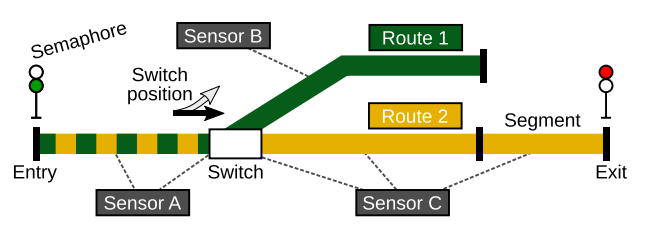
\includegraphics[width=0.7\textwidth]{figures/trainbenchmarkfig1}
	\caption{Vasúti útvonal részlet (forrás: \cite{szarnyas2018train})}
	\label{fig:trainbenchmark}
\end{figure}

 \Aref{fig:trainbenchmark}-es ábrán látható egy a trainbenchmark metamodelljére alapuló részlet. Ebben a kontextusban egy vasúti útvonal nem más mint szegmensek és váltók sorozata, illetve a belépést és a kilépést egy-egy szemafor jelzi. Ahhoz hogy biztonságos legyen a közlekedés szükség van szenzorokra, amelyek monitorozzák a különböző szegmensek és váltók kihasználtságát. Egy útvonal definiálásához ,a felsorolt elemeken kívül a váltók adott útvonalhoz tartozó pozícióját is el kell tárolnunk. Egy útvonal akkor aktív, ha a rendszerben a specifikációjának megfelelően állnak a váltók.

A metamodellezés egy tecknika arra, hogy definiájunk modellező nyelveket, ahol a metamodell specifikálja a nyelv szintaktikáját. A trainbenchmark metamodellje \aref{fig:trainbenchmarkmetamodell} -es ábrán látható.

\begin{figure}
	\centering
	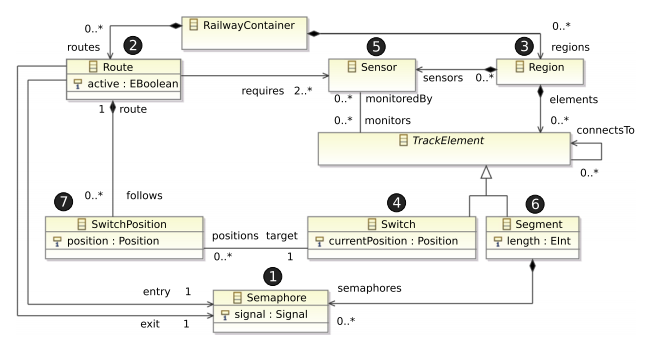
\includegraphics[width=0.7\textwidth]{figures/trainbenchmarkfig2}
	\caption{A train benchmark metamodellje. a, tartalmazási hierarchia és relációk b, öröklési relációk (forrás: \cite{szarnyas2018train})}
	\label{fig:trainbenchmarkmetamodell}
\end{figure}


\section{Gráflekérdező rendszerek}
A gráfok intuitív formalizációt nyújtanak modellezési szempontból arra, hogy úgy írhassuk le a világot ahogy az ember gondolkozik róla. Tehát mint dolgok (csomópontok) és köztük lévő kapcsolatok (élek) \cite{marton2017model}. A property gráf adatmodell kiterjeszti a gráfokat úgy, hogy címkéket/típusokat illetve tulajdonságokat ad a csúcsoknak és az éleknek. A gráf adatbázisok  alkalmasak tulajdonság gráfok tárolására, és az abban lévő adatok lekérdezésére komplex gráf minták használatával. Ilyen rendszerek például a    Neo4j \cite{neo4j}, OrientDB \cite{orientdb} és a  SparkSee \cite{sparksee}.

\begin{figure}
	\centering
	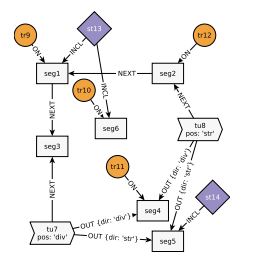
\includegraphics[width=0.7\textwidth]{figures/tulajdonsággráfpélda}
	\caption{Property gráf példa(forrás: \cite{marton2017model})}
	\label{fig:tulajdonsággráfpélda}
\end{figure}

Ahhoz hogy jobban megérthessük mi is ez az adatmodell \aref{fig:tulajdonsággráfpélda} -es ábrán látható egy példa.
\subsection{Neo4j}




\section{Modellezés és metamodellezés}
\subsection{Cypher query-k metamodellje}
\subsection{xText}
\subsection{\textsc{Viatra} jólformáltsági kényszerek}

\section{Gráfgenerálás}

ábra milyen bemenetek milyen kimenetek






\chapter{\attekintes}

\section{Funkcionális áttekintés}

Munkám célja hogy elkészítsek egy olyan megközelítést, amely képes gráflekérdezések automatikus generálására, gráfmintaillesztő rendszerek tesztelése. Az elképzelt  keretrendszer koncepcionális elrendezését  \aref{fig:funkcionalisAttekintes} ábrán mutatom be. Az ötlet lényege az, hogy a tesztelni kívánt rendszer \textbf{nyelvi specifikációjának} és egy \textbf{esettanulmány szignatúrájának} (ezalatt egy olyan tulajdonsággráf adatmodell alapú adatbázis szignatúrájára gondolok amely az adott lekérdező rendszert használja) bemenetként való felhasználásával, a kimeneten szöveges és a gráfmintaillesztő rendszer nyelvén íródott lekérdezéseket kapjak. 

Amint rendelkeznék egy tesztkészletnyi ilyen lekérdezéssel azokat tudnám futtatni azon az adatbázison amelynek szignatúráját esettanulmányként választottam. Ha az ezzel a módszerrel generált lekérdezésekre adott válaszok válaszidejeit összehasonlítjuk több rendszeren tudnánk \textbf{teljesítményben tesztelni} azokat. Illetve ha a generált lekérdezések helyes eredményével is rendelkeznénk, (például több létező implementációt összehasonlítanánk, és egyiket a másik referenciájaként használnánk, akkor a referencia  megfelelő tesztorákulumként szolgálhatna, így ellenőrizni tudnánk azt is hogy a teszt alatt álló lekérdező rendszer hogyan funkcionál, helyes válaszokat ad-e? Ha elég bonyolultak a lekérdezések, akkor az is lehetséges, hogy lesznek olyanok amelyek az egyes lekérdező motorokon nem míg másikakon működnek, így azt is \textbf{tesztelni} tudnánk hogy mekkora az egyes lekérdező motorok funkcionális lefedettsége.
\todo{bekezdés ami Oszkárnak kell}
    
Felmerül a kérdés, hogy mégis miért lesz ez jobb, mintha írnánk a lekérdezéseket magunk. Azért, mert a generálás segítségével ki tudunk törni az emberi sematikus gondolkozásból, és olyan lekérdezéseket tudunk készíteni amelyek számításokkal bizonyítottan különböző ekvivalencia osztályba tartoznak. Az ekvivalencia partícionálás, egy bevett  technika tesztelésnél \cite{burnstein2006practical}, mérésekkel bizonyították, hogy a generált modellek szignifikánsan magasabb tesztfedettséget mutattak, mint a manuálisan elkészítettek \cite{semerath2018iterative}. Illetve nem korlátoz minket az sem, hogy a teszteléshez írt lekérdezésekből túl kevés van, mert a generátor segítségével megadott számú minta, akár óriási tesztkészlet előállítható automatikusan.

A megközelítésemet egy Neo4j \cite{neo4j} property gráf adatbázison mutatom be, amely a Train benchmark \cite{szarnyas2018train} által használt szignatúrával van felszerelve. A  lekérdezéseket a Neo4j által kifejlesztet Cypher \cite{Cypher} nyelven generálom, a slizaa \cite{slizaa_2018} által készített openCypher nyelvi specifikáció felhasználásával. 


\begin{figure}
	\centering
	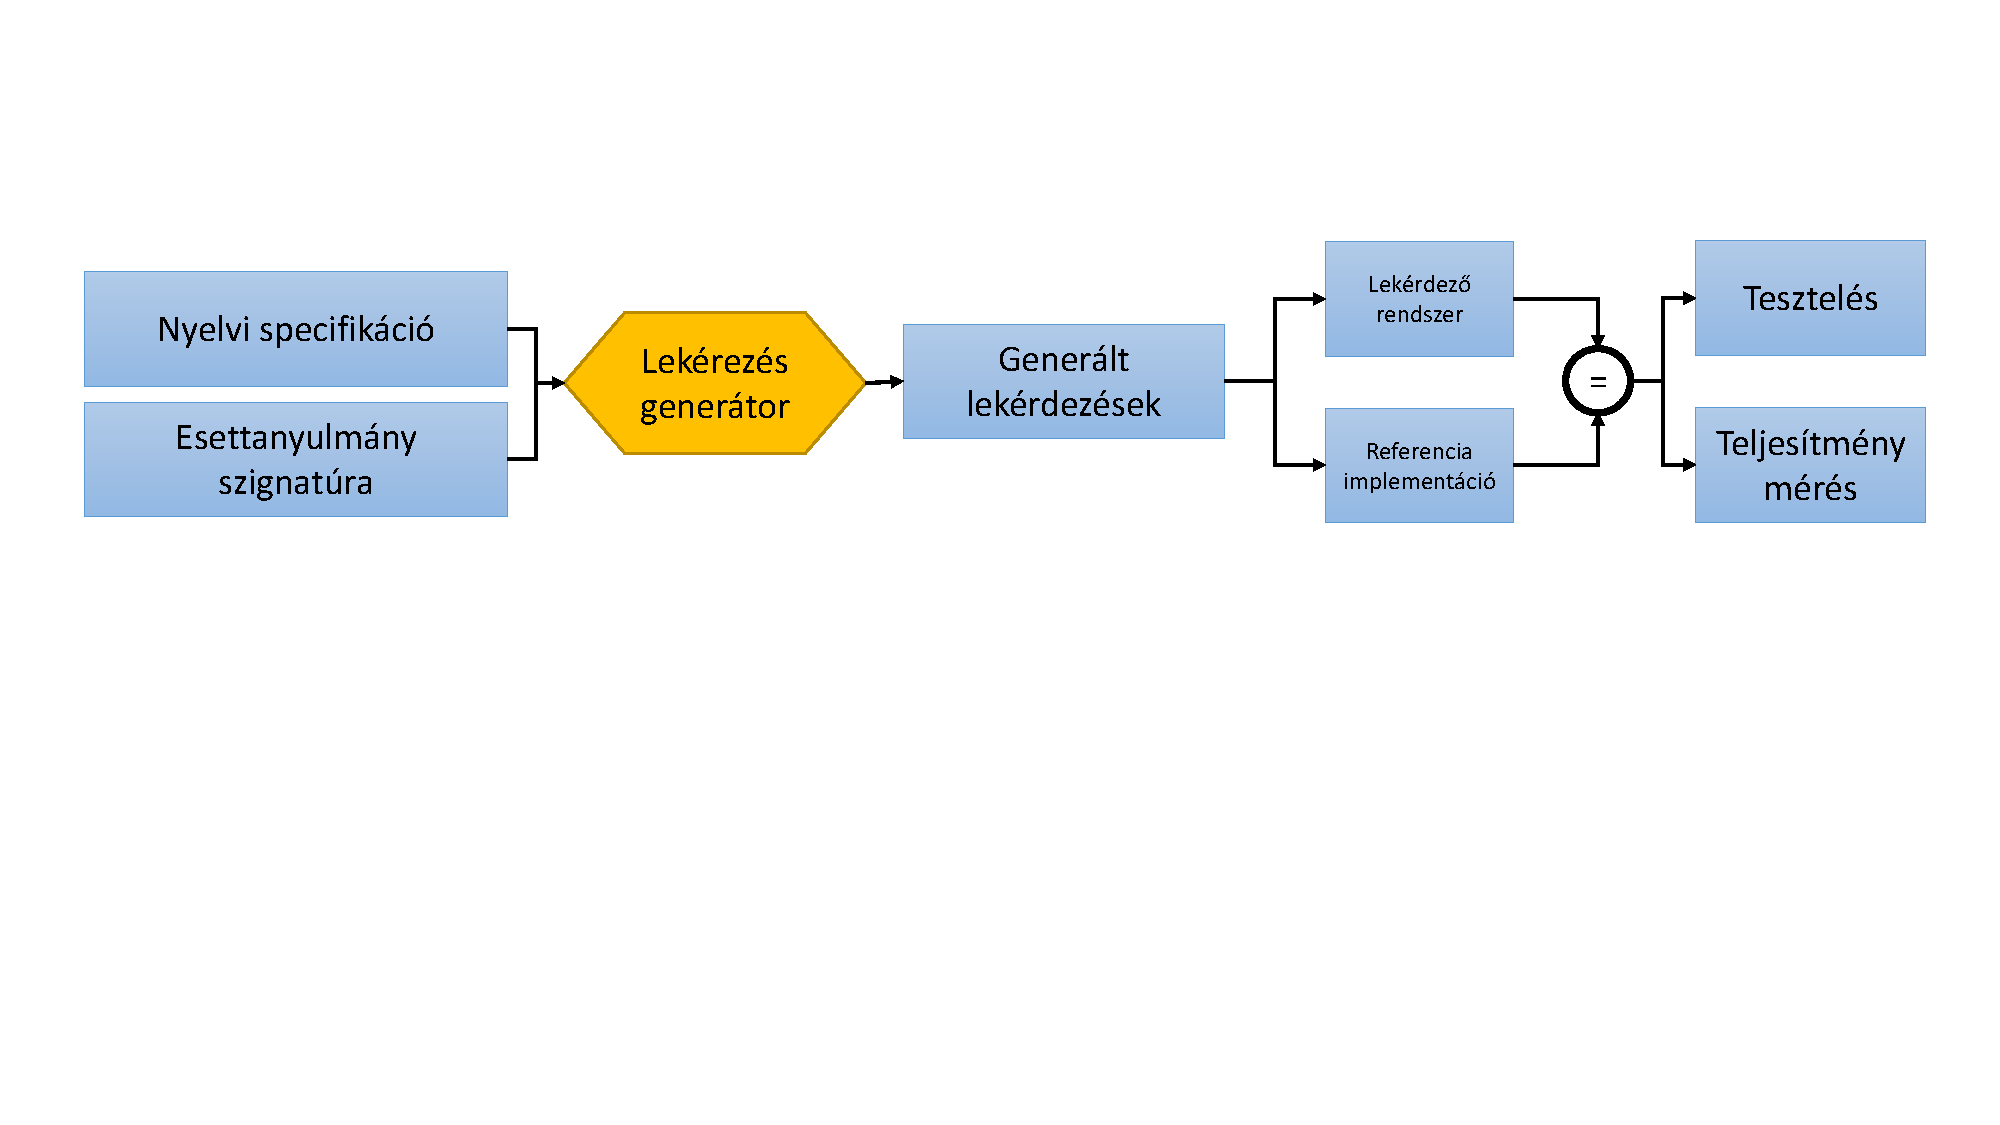
\includegraphics[width=1.0\textwidth]{figures/funkcionalisAttekintes}
	\caption{Az elképzelés funkcionális áttekintése}
	\label{fig:funkcionalisAttekintes}
\end{figure}
 
  

\section{Lekérdezés generálási folyamat felépítése}


A folyamat felépítését \aref{fig:blokkdiagramAttekintes} -es ábra segítségével ismertetem.  

\begin{figure}
	\centering
	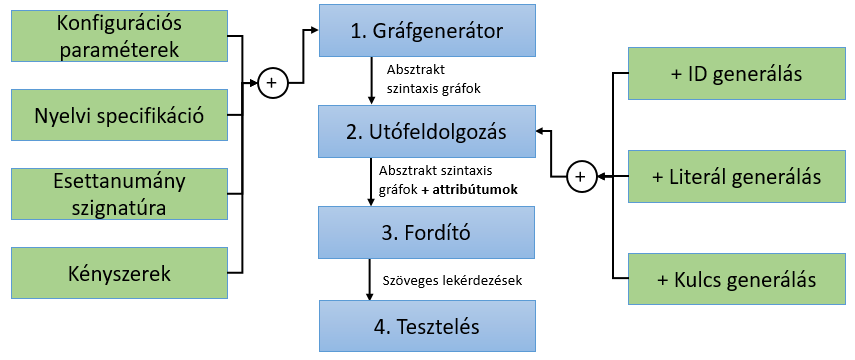
\includegraphics[width=1.0\textwidth]{figures/blokkdiagramAttekintes}
	\caption{A lekérdezés generálási folyamat áttekintése}
	\label{fig:blokkdiagramAttekintes}
\end{figure}
\begin{enumerate}
	\item \textbf{Gráfgenerátor}
	A gráf generálást a Viatra Solver keretrendszer  segítségével végzem. Ehhez sok különböző bemenetet kell megadnom. 
	\begin{enumerate}
		\item\textbf{Nyelvi specifikáció}: A Cypher nyelv specifikációját tartalmazó metamodell a nyelv egészére kiterjed. Így lekérdezéseken kívül sok egyéb műveletet is definiál, mint például létrehozás, törlés. Olyan kényelmi, extrafunkcionális elemeket is tartalmaz amelyek csak bonyolítják a lekérdezéseket, hogy felhasználóbarátabban adhassák vissza a tartalmat, például a visszatérési referencia átnevezése \cypherStyle{(x AS "username")}. Ahhoz, hogy egyszerű lekérdezéseket generáljak nem szükséges ezt a hatalmas metamodellt feldolgozni, viszont egyértelműen meg kell határozni egy olyan részmodelljét, amelyből hiánytalanul előáll az egyszerű lekérdezések nyelvi specifikációja, továbbá a lényegtelen elemek szűrésével a generált modellsereg diverzitását is növeljük, mert így lényeges modellelemek között kell hogy különbözzenek. 
		\item\textbf{Kényszerek}:Azonban vannak	olyan szabályok amelyeket a metamodell nem tud kifejezni, betartásuk nélkül viszont a generált példánygráfok nem értelmezhetőek Cypher nyelvű lekérdezésekként. Például annak meghatározása, hogy milyen változókra lehet, és milyenekre nem lehet hivatkozni a visszatérési értékben. Ezeket a szabályokat jólformáltsági kényszerekkel tartatom be. 
		\item\textbf{Konfigurációs paraméterek}: A generátor működéséhez elengedhetetlen a saját nyelvén íródott konfigurációs fájl. Itt határozható meg, hogy milyen megoldóval működjön a generálás, hogy hányat használjon az egyes elemekből a generálás során, hogy mekkora és milyen mennyiségű példányokat generáljon stb.  
		\item\textbf{Esettanumány szignatúra} : A generált példánygráfok változók nélkül jönnek létre. Ahhoz, hogy egy értelmes adatbázison végezhessük el őket, fontos hogy fel legyenek fegyverezve az adatbázisban használt címkékkel, típusokkal. Mivel én a Train Benchmark által használt adatbázison futtattam lekérdezéseimet, ezért az általa használt szignatúrával szereltem fel a rendszert. 
	\end{enumerate}
	\item \textbf{Utófeldolgozás} : Az általam generált gráfokban a változóknak nem adok nevet. Megtehetném, hogy a generálás során kitöltöm őket, de csak úgy, hogy a gráfgenerátor a generált szavakat különbségekként kezelje két példánygráf között. A nagyobb diverzitás elérésének érdekében a generátor nem foglalkozik a változók elnevezésével. Az utófeldolgozás során az Esettanulmány szignatúra szavaival töltöm fel az addig még csonka példánygráfokat.    
	\item \textbf{Fordító} : Az utófeldolgozás során sorosíthatóvá vált példány gráfokat a Cypher nyelv XText nyelven íródott nyelvtanának segítségével szöveges lekérdezésekké alakítom.  
\end{enumerate}




\chapter{Gráflekérdezések automatikus generálása}
\label{chp:4}

\section{Lekérdezések generálása}

\subsection{Tesztelni kívánt résznyelv kiválasztása}

A gráfgenerátor egyik bemenete a tesztelni kívánt nyelvi fregmens metamodellje. Ahhoz, hogy hasznos tesztesetek állítsunk elő, szükséges a generátort egy konkrét feladatot ellátó modellek előállítására konfigurálni. (Ha az egész nyelvet használnánk akkor a lekérdezése érdektelen részletekből állna, például kommenteket, felesleges változó átnevezéseket, lekérdezéssel kapcsolatos metainformációkat generálna.) Munkám során tehát az első feladat az, hogy kiválasszam a Cyphernek egy olyan releváns résznyelvét amellyel tesztelés szempontjából releváns lekérdezéseket lehet generálni. Dolgozatomban olyan úgynevezett pozitív mintájú lekérdezések generálására koncentrálok, amelyek vizsgálják a csomópontok illetve a csomópontok közötti kapcsolatok típusát és attribútumait. Ugyanis számos lekérdező nyelvben, mint például Cypher \cite{Cypher} és \textsc{VIATRA} \cite{viatra} ezek képezik a lekérdezések alapját. 

%Dolgozatomban az alábbihoz hasonló lekérdezések generálásával foglalkoztam 
%
%\begin{lstlisting}[style=cyphersmall]
%MATCH (train : Train {name : "train1"})-[:ON]->(seg : Segment {name : "seg3"}) 
%RETURN seg
%\end{lstlisting}


Alább azt kívánom megmutatni, hogy milyen módszerrel lehet le szűkíteni egy Xtext alapú Cypher metamodellt. 

\begin{enumerate}
	\item  Példalekérdezések kiválasztása, amelyekhez hasonló tesztkészletet szeretnék generálni.
	\item  Példákból ASG-k készítése.
	\item  ASG-kból legnagyobb közös részgráf előállítása: ez fogja  alkotni a kiindulási részmodellt.
	\item  ASG-kben használt összes nyelvi konstrukció (típusok, referenciák, literálok) összegyűjtése: ez adja az effektív metamodellt.
\end{enumerate}   


\subsection{Jólformáltsági kényszerek betartása}
A gráfgenerátor másik bemenete olyan kényszerek halmaza, amelyek szükségesek ahhoz, hogy értelmes modelleket tudjunk generálni. Ezekre főleg azért van szükség, mert az Xtext-ben \cite{xText} íródott nyelvtan és a nyelvtan metamodellje közötti konverzió nem tökéletes. Jólformálsági kényszerekre azért van szükség, mert nem minden a metamodellel leírható modell sorosítható Cypher nyelvű lekérdezéssé. Ennek több oka is van: (1) A precíz metamodell meghatározása számításilag komoly kihívást jelent és nem is végezték el a keretrendszer megalkotói, (2) A metamodellnek hibás modellek leírására is alkalmasnak kell lennie (hiszen szerkesztés közben általában félkész modellek vannak a rendszerben) (3) A metamodell a modelleknek csak az alap struktúráját (referencia hova mutathat) írja le, bonyolultabb szabályok (összetett logikai kifejezések) meghatározására alkalmatlan.
 Az Xtext Cypher nyelvtanban leírt parseolhatósági szabályokat át kell fordítani ASG-n értelmezett struktúrális kényszerekké. 






A lenti kényszer azt határozza meg, hogy a lekérdezésekben a \cypherStyle{RETURN} szó után kötelező legalább egy változóra referálni. A felső minta meghatározza, hogy hogyan néz ki egy olyan \viatraStyle{ReturnItem} aminek van \viatraStyle{VariableRef} a visszatérési értékében. Az alsó pedig egy kényszer, aminek felírásával garantálom, hogy csak olyan eredmény áll elő, ahol a hiba-minta nem teljesül.


\begin{lstlisting}[style=viatrasmall]
pattern hasReference(retI : ReturnItem, variRef : Expression){
	VariableRef(variRef);
	ReturnItem.expression(retI, variRef);
}

@Constraint(severity ="error", key={ri}, message = "error")
pattern hasNoReference(ri : ReturnItem){
	neg find hasReference(ri, _);
}
\end{lstlisting}
Minden \viatraStyle{Pattern}-nek kell hogy legyen legalább egy \viatraStyle{PatternElement}-je. Ezt a lenti kényszerben fogalmazom meg. A kényszerre a konzisztens és hatékonyabb generálás érdekében van szükség. (Egy \viatraStyle{Pattern}-be a nyelvtan alapján \viatraStyle{.patterns} tulajdonság beállításakor más elem  is kerülhetne, de a  tesztkészletet generálásához felhasznált példalekérdezések között egyéb elemre nem volt példa.) 

\begin{lstlisting}[style=viatrasmall]
pattern wellLookingPattern (patt : Pattern, patternElement : PatternElement){
	Pattern.patterns(patt,patternElement);
}
@Constraint 
pattern notWellLookingPattern(patt : Pattern){
	neg find wellLookingPattern(patt , _);
}
\end{lstlisting}


A lenti két kényszer megtiltja, hogy egy \viatraStyle{PatternElement} rendelkezzen \viatraStyle{var} és  \viatraStyle{part} tulajdonságokkal. Ilyen tulajdonsága csak a \viatraStyle{PatternPart} osztálynak lehetnek, de a nyelvtan metamodellje alapján helytelenül a \viatraStyle{PatternElement} osztály is megörökli őket. 

\begin{lstlisting}[style=viatrasmall]
@Constraint
pattern  patternElementHasVar(pE : PatternElement, vari: VariableDeclaration){
	PatternElement.^var(pE,vari);
}

@Constraint
pattern  patternElementHasPart(pE : PatternElement, pp : PatternPart){
	PatternElement.part(pE,pp);
}
\end{lstlisting}

Az alábbi kényszerben megfogalmazom, hogy ne legyen \viatraStyle{PatternPart} a generált csomópontok között, hanem mindig \viatraStyle{PatternElement}-ek jöjjenek létre. Erre azért van szükség, mert a metamodellben mindkét osztály szerepel, és egyik sem absztrakt. A kényszer által jelentősen csökken a generátor futásideje.

\begin{lstlisting}[style=viatrasmall]
pattern pe(pe:PatternElement) {
	PatternElement(pe);
}

@Constraint
pattern notPatternElement(pp : PatternPart){
	neg find pe(pp);
}
\end{lstlisting}


A \viatraStyle{Mapliteral}-ok a következőképpen néznek  ki a Cypher nyelven: \cypherStyle{ name : "seg3"}, egyéb elemek nem kerülhetnek bele. A \viatraStyle{Mapliteral} osztály ennek ellenére helytelenül örököl egy \viatraStyle{nodelabels} tulajdonságot is. A lenti kényszer biztosítja hogy ne töltse ki azt.

\begin{lstlisting}[style=viatrasmall]
@Constraint
pattern notWellLookingMapliteral(mapLiteral : MapLiteral, nodeLabel: NodeLabel){
	MapLiteral.nodeLabels(mapLiteral,nodeLabel);
}

\end{lstlisting}

Erre a mintára pedig azért van szükség, mert ha nem lenne akkor a következőhöz lekérdezéshez hasonló értelmetlen lekérdezések generálása válna lehetővé és a generátor nagy méretű modelleknél könnyen esne abba a hibába, hogy az extra csúcspontokat így pocsékolja el.


\begin{lstlisting}[style=viatrasmall]
pattern wellDeepMap(mapLiteralEnrty: MapLiteralEntry, string : StringLiteral){
	MapLiteralEntry.value(mapLiteralEnrty,string);
}

@Constraint
pattern notWellDeepMap(mapLiteralEnrty : MapLiteralEntry){
	neg find wellDeepMap(mapLiteralEnrty, _);
}
\end{lstlisting}



\begin{lstlisting}[style=cyphersmall]
MATCH (seg : Segment {name : {name2 : {name3: { name4 : seg4}}}}) 
RETURN seg
\end{lstlisting}



\subsection{Diverzitás biztosítása}
A generált modellszekvencia használhatatlan lenne, ha a lekérdezések között nem, vagy csak lényegtelen különbségek lennének. Dolgozatomban több féle szinten is garantálom a lekérdezések diverzitását (elkerülve ezzel hogy túlságosan hasonló lekérdezések szülessenek). A diverzitás biztosítása kiemelten fontos tesztgenerálási feladatoknál, mert így hatékony ekvivalencia partícionálást biztosíthatunk. Generálás során az alábbi lényegi különbségeket garantáljuk.

\begin{itemize}
	\item Egyenértékű változók elnevezésétől függetlenül azonosnak találjuk az alábbi két megoldást, hiszen a válasz a két lekérdezésre azonos értékeket adna vissza.
\begin{lstlisting}[style=cyphersmall]
MATCH ( V1 : Segment  )-->( V2 : Segment ) RETURN V1 , V2
MATCH ( Var1 : Segment  )-->( Var2 : Segment)	RETURN Var1 , Var2
\end{lstlisting}
	\item A változók sorrendezésétől függetlenül azonosnak tekintjük az alábbi két problémát, hiszen a két lekérdezés ugyanazt a táblázatot adná vissza csupán az oszlopokat fordított sorrendben jelenítené meg.
\begin{lstlisting}[style=cyphersmall]
MATCH ( V1 : Segment  )-->( V2 : Segment ) RETURN V1 , V2
MATCH ( V1 : Segment  )-->( V2 : Segment ) RETURN V2 , V1
\end{lstlisting}
	\item A attribútomok ellenőrzésének sorrendje nem számít, hiszen ugyanannak a csomópontnak attribútumairól van szó, mindegy milyen sorrendben írjuk.
\begin{lstlisting}[style=cyphersmall]
MATCH ( Var1 : Segment { signal : "String1", currentPosition : "String2" }) 
RETURN Var1
MATCH ( Var1 : Segment { currentPosition : "String2", signal : "String1" })
RETURN Var1
\end{lstlisting}
	\item Illetve a vesszővel elválasztott minta részek sorrendje sem változtat a lekérdezés eredményén, mert ezek metszetét értékeli ki a lekérdező rendszer.  
\begin{lstlisting}[style=cyphersmall]
MATCH ( V1 : Segment { signal : "String1"} ) , 
	  ( V2 : Route { length : "String2" } )
RETURN V1 ,V2
MATCH ( V2 : Route { length : "String2" } ) ,
	  ( V1 : Segment { signal : "String1"} )  
RETURN V1 ,V2
\end{lstlisting}
\end{itemize}

A fenti példák nem tartalmaznak lényegi szűrést, továbbra is az összes lehetséges lekérdezés generálható marad.

Továbbá az alábbi extra diverzitást is biztosítottam a lekérdezések létrehozása során:
\begin{itemize}
	\item Két struktúrálisan hasonló lekérdezést nem különböztetünk meg. Struktúrálisan hasonlónak azokat a lekérdezéseket tekintem amelyek a típusnevek átírásával azonossá válnának.
\begin{lstlisting}[style=cyphersmall]
MATCH ( V1 : Segment  )-->( V2 : Segment ) RETURN V1 , V2
MATCH ( V1 : Route  )-->( V2 : Switch ) RETURN V1 , V2
\end{lstlisting}
	\item A literál értékeket is hasonlónak tekintjük az előző ponthoz hasonlóan ez is a struktúrális különbségek létrehozásnak érdekében történik. 
\begin{lstlisting}[style=cyphersmall]
MATCH ( Var1 : Segment { signal : "String1" }) RETURN Var1
MATCH ( Var1 : Segment { signal : "String2" }) RETURN Var1
\end{lstlisting}
	\item A generátoron belül a diverzitás szintet magasra állítottam. Ez aszerint növeli a különbségeket két gráf között, hogy megvizsgálja a csomópontok szomszédságát ( a csomóponttal szomszédos csomópontok halmaza). És nem generál több, csak azonos szomszédságokból álló gráfot.  
\end{itemize}


\section{Utófeldolgozás}
Az előző fejezetben megoldottam a modellek lényegi részeinek generálását, amely biztosította hogy a modellek lényegi különbségekkel rendelkezzenek. Ezt a feladatrészt az utófeldolgozás során végzem el. Itt adom hozzá ezen kívül azokat a részleteket is a modellekhez, ami mindegyikben azonos, ezért a generálás során nem foglalkoztam vele. 

Ahhoz, hogy értelmesen nevezzem el az egyes változókat, a Train Benchmark-ban használt kifejezéseket és értékeket osztom ki, amik láthatóak \aref{fig:trainbenchmarkmetamodell}. ábrán. Három féle elemet kell elneveznünk a jelenleg generált modellekben. (1) csomópont címkék \viatraStyle{NodeLabel.labelName} , (2) kapcsolat címkék \viatraStyle{RelationshipDetail.relTypeNames} és (3) tulajdonság címkék \viatraStyle{MapLiteralEntry.key}.
Ezek mind megfeleltethetőek \aref{fig:trainbenchmarkmetamodell}. ábrán látható elemeknek. A csomópont címkék az osztályok neveinek, a kapcsolat címék az asszociációk neveinek, míg a tulajdonságcímkék az attribútumoknak. Ezért készítettem három listát a megfelelő nevekkel.
\begin{enumerate}
	\item csomópont címkék: \cypherStyle{Region}, \cypherStyle{Route}, \cypherStyle{Segment}, \cypherStyle{Semaphore}, \cypherStyle{Sensor}, \cypherStyle{Switch}, \cypherStyle{SwitchPosition}
	\item kapcsolat címkék: \cypherStyle{connectsTo}, \cypherStyle{entry}, \cypherStyle{exit}, \cypherStyle{follows}, \cypherStyle{monitoredBy}, \cypherStyle{monitors}, \cypherStyle{requires}, \cypherStyle{target}
	\item tulajdonság címkék: \cypherStyle{id}, \cypherStyle{active}, \cypherStyle{position}, \cypherStyle{currentPosition}, \cypherStyle{length}, \cypherStyle{signal}
	
\end{enumerate}
Ezután szükségem volt egy randomizáló függvényre, amely a megfelelő nevek valamelyikét elhelyezi egy-egy elemen.
Majd bekötöttem mindhárom típus minden elemére a megfelelő szavakat. Ezen kívül a lekérdezésekben vannak változók is amelyeket szisztematikusan elneveztem \cypherStyle{V1...Vn}-el, illetve literálok amiket pedig \cypherStyle{"String1"..."Stringn"}-el neveztem el. 

Fontos megjegyezni, hogy a generált lekérdezéseknek a konkrét Train Benchmark modelleben nem mindig lesz megoldása. Nézzük meg az alábbi példát:
 \begin{lstlisting}[style=cyphersmall]
 MATCH ( Var1 : Segment { signal : "String1" })
 RETURN Var1 \end{lstlisting}
 \noindent Hiszen a Train Benchmark metamodellje alapján egy szegmensnek nincsen signal tulajdonsága, tehát egy metamodell alapján felépített gráf adatbázisban nem találnánk a lekérdezésben szereplő mintát. A Neo4j gráfadatbázisára viszont igaz, hogy nem típusos, így nem készülhet fel a modell alapvető struktúrájára. Ha akarnánk bele tudnánk írni egy olyan csomópontot, ami Segment címkét kap és signal tulajdonsággal rendelkezik, és a felhasználókat semmi nem akadályozza meg abban, hogy esetleg értelmetlen gráfadatbázist hozzanak létre. Így amikor keresünk egy ilyen adatbázisban fel kell hogy legyen készülve arra, hogy olyan dolgot keresünk amit nem találhatunk meg. 

\section{Fordítás}

A generált gráfokat az utófeldolgozás után kifejezések  ASG-jeként értelmezem, majd a nyelvtani szabályok fordított irányú alkalmazásával szöveges dokumentummá alakítom. A fordító a szöveggé alakítás során szóközöket rak a szükséges helyekre, behelyettesíti a változók neveit a rájuk mutató referenciákba,  kitölt a nyelvtani szabályokban meghatározott szavakat pl: \cypherStyle{MATCH , RETURN} , illetve megfelelő helyekre  zárójeleket rak. A fordítást az Xtext keretrendszerének segítségével automatizálom.


\chapter{\evaluation}
\label{chp:5}

Ebben a fejezetben kiértékelem munkámat mialatt megválaszolom a következő kérdéseket:

\begin{itemize}
	\item \textbf{Kérdés1}: Hogy aránylik egymáshoz az előfeldolgozás, a generálás és az utófeldolgozás időtartama?
	\item \textbf{Kérdés2}: Hogy skálázódik a generálás lekérdezés méretének szempontjából?
	\item \textbf{Kérdés3}: Hogy skálázódik a generálás lekérdezés darabszámának szempontjából?
	\item \textbf{Kérdés4}: Mennyire diverzek a lekérdezések a tesztelés minőségének szempontjából?
	\item \textbf{Kérdés5}: Milyen eredménnyel futtathatóak a lekérdezések egy Neo4j gráfadatbázison?
\end{itemize}

\section{Mérési környezet felállítása}


A méréseket eclipse fejlesztői környezetben végeztem. Ahhoz, hogy bemelegítsem a modell generátort memóriakezelés és optimalizálás szempontjából 5 extra futást adtam hozzá minden kiértékelt mérés előtt, melyek futásidejét a mérés során figyelmen kívül hagytam. A mérésekhez a generátor számára 4000 MB memóriát biztosítottam, és ez mindig elegendőnek bizonyult. Az összes mérést egy egyszerű asztali számítógépen végeztem (Intel Core i7-3520M CPU, 2.90GHz, Windows 10 Pro). A generáláshoz részmodellként egy 22 elemből álló ASG-t adtam meg, de csak az esszenciális részletek specifikálásával. Erre az alapra építve két különböző mérési környezetet implementáltam, hogy mind a 4 kérdésre választ tudjak adni. A két környezetben generált gráfok elkészültük után egy utófeldolgozás fázison mentek keresztül, ahol Cypher nyelvű lekérdezésekké fordítottam le őket.

\subsection{M1: Skálázódás modellkészlet méretében}

Az első mérési környezetben 50-50 eltérő lekérdezést generáltam, úgy, hogy 10 20 és 30 elemmel egészítettem ki a kiindulási állapotot. Minden mérést 10-szer megismételtem (a belemelegedést leszámolva). Az elrendezés célja, hogy a generátor skálázhatóságát vizsgálja modellkészlet méretének szempontjából.

\subsection{M2: Skálázódás modellkészlet méretében} 
A második  mérési környezetben 10-10 eltérő lekérdezést generáltam, 5, 10 ,15, ...,50, 100, 150, 200 elemmel egészítettem ki a kiindulási állapotot. Minden mérést 10-szer megismételtem (a belemelegedést leszámolva). Az elrendezés célja, hogy a generátor skálázhatóságát vizsgálja modellek méretének szempontjából.


\section{A futásidő összetétele}

\begin{figure}[htp]
	\centering
	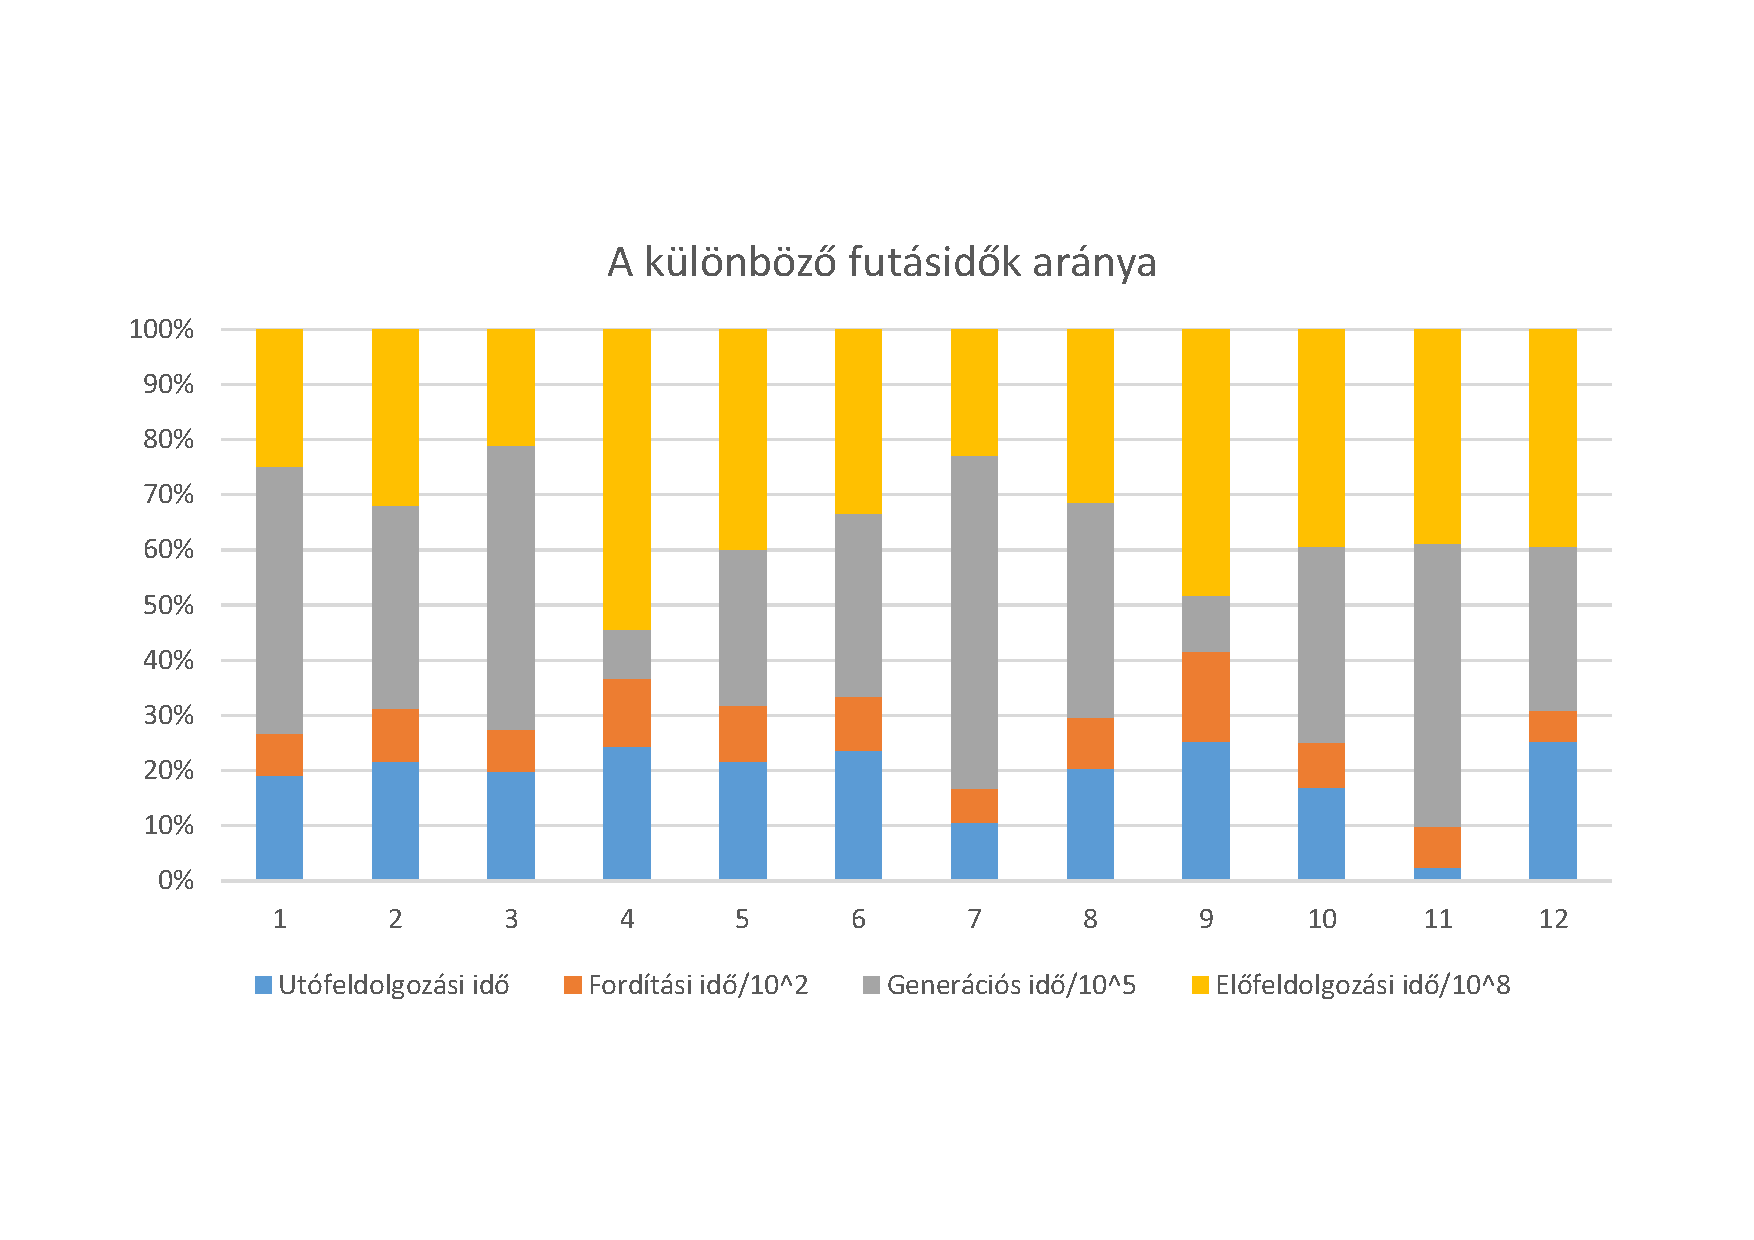
\includegraphics[width=1\textwidth]{figures/aránygrafikontáblázathelyett}
	\caption{A K1 mérés eredményei}
	\label{fig:grafikon}
\end{figure}

A futásidő összetételének vizsgálatát az M1 mérési környezetben végeztem el, de M2 esetén is hasonló karakterisztikát mutat. A mérés eredményei  \aref{fig:grafikon}. ábrán láthatóak. Az ábra segítségével azt szeretném bemutatni, hogy a különböző futásidők nagyságrendileg mekkora részét képezik a futásidő egészének. A három szín három értéket reprezentál: az előfeldolgozás idejét (ide tartozik a modellezési nyelv beolvasása, leképezése logikai feltételekké, a logikai probléma megfelelő formára hozása) kék színnel, a generálás idejét (ide a VIATRA Solver futása tartozik) szürke színnel, az utófeldogozás idejét (logikai probléma értelmezése, gráfként való ábrázolása, utófeldolgozás, változók és literálok elnevezése, végül a megoldás gráf ASG -ként való értelmezése és szöveggé alakítása) pedig narancssárga színnel jelölöm. (Alulról felfelé kék, szürke, narancs.) A grafikon vízszintes tengelye a teljes futásidőt mutatja meg. Az első oszlop a 10 a második a 20 a harmadik pedig a 30 hozzáadott csomópontban minimalizált al-környezetben végzett mérések futásidejének összegét ábrázolja. 

Az ábrán látható, hogy míg az elő és az utófeldolgozás összes ideje nem mutat jelentős különbséget a három esetben, addig a generálás időtartama szignifikánsan különbözik. Láthatóan a legkisebb méretnél a leghosszabb és a legnagyobbnál a legrövidebb. (Ennek az okát következő szekcióban fejtem ki.)

\textit{Végeredményben levonhatom a következtetést, hogy a futásidő leghosszabb részét a generálás ideje teszi ki, míg az előfeldolgozás és az utófeldolgozás arányaiban megegyező időtartamú, kisebb modellek esetében az előfeldolgozás, nagyobbak esetében pedig az utófeldolgozás tart tovább.}   

\section{Skálázódás a modellek méretének függvényében}

\begin{figure}[htp]
	\centering
	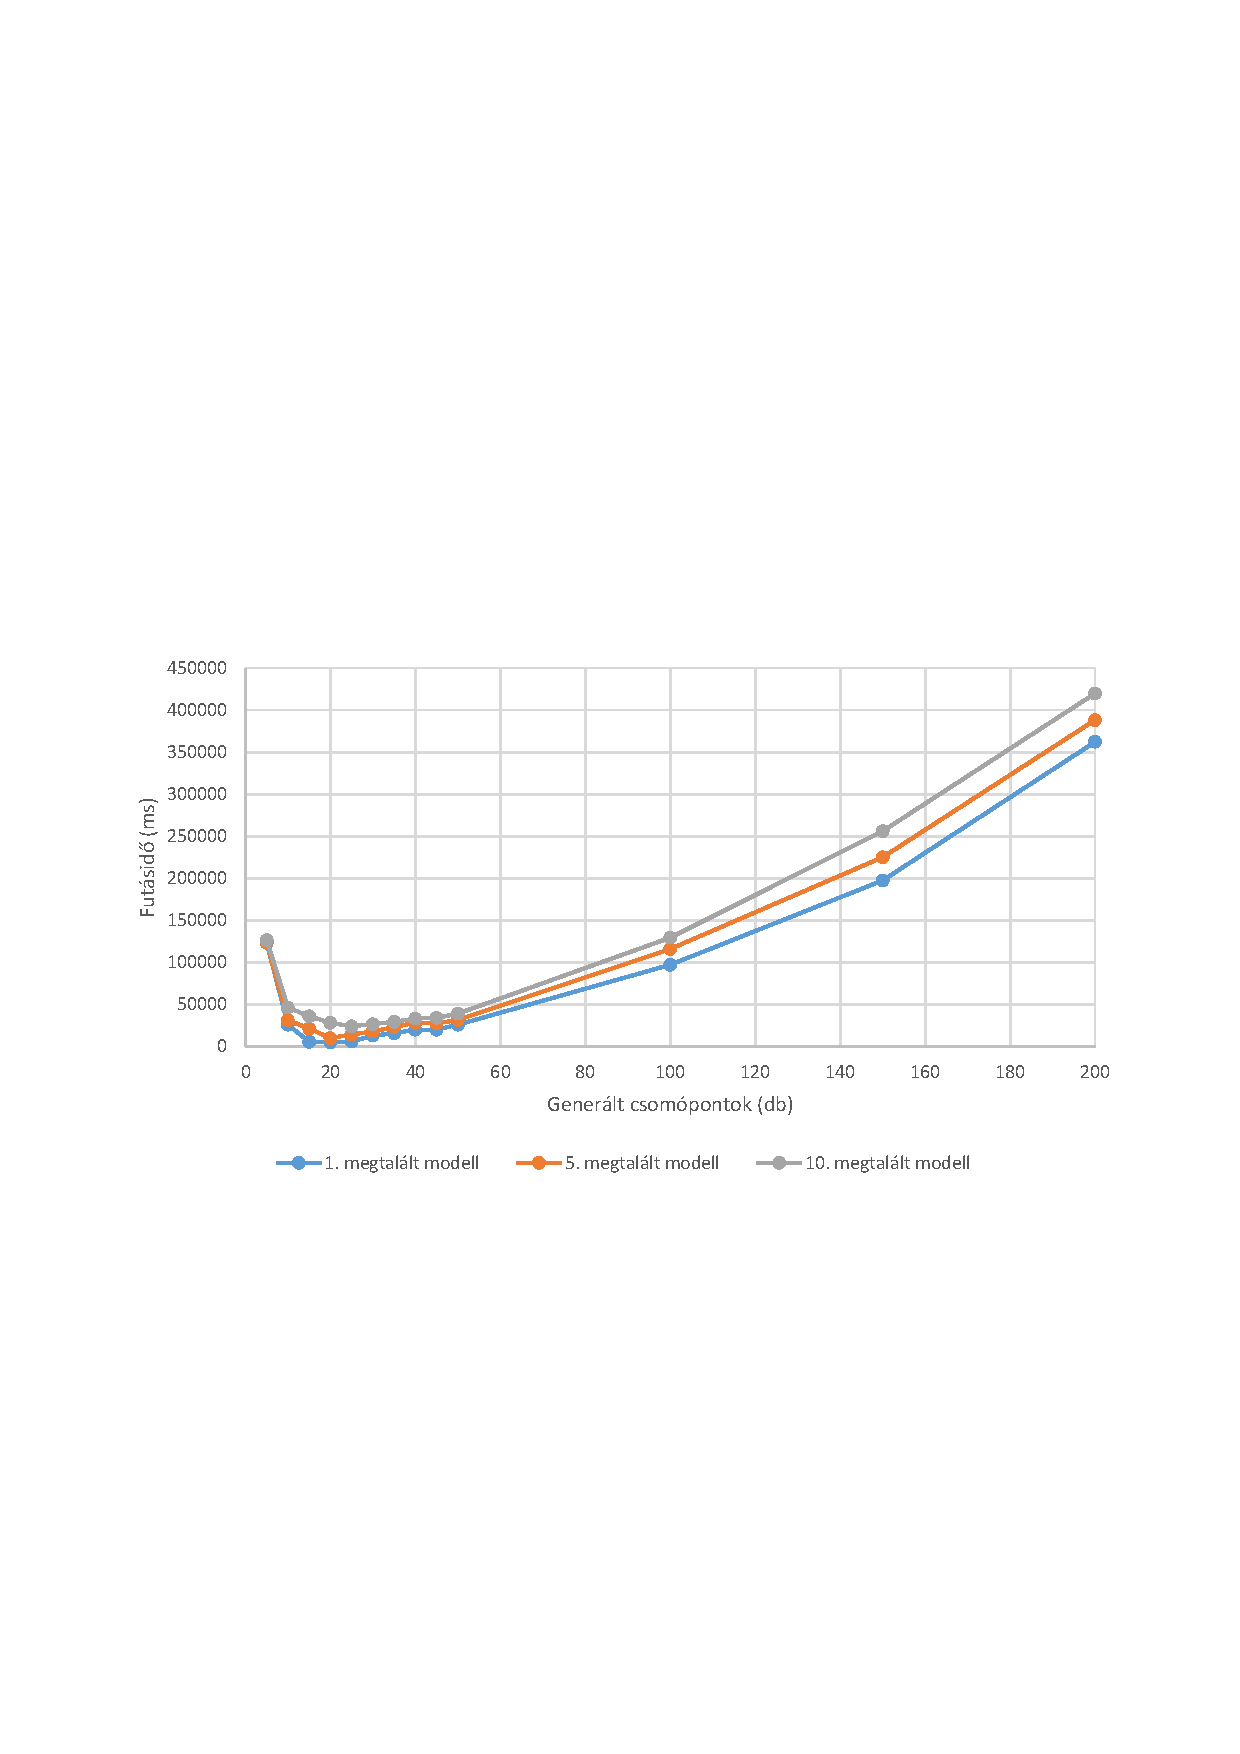
\includegraphics[width=1\textwidth]{figures/statisticsPlottal1}
	\caption{A K2 mérés eredményei}
	\label{fig:BmeresEredmeny}
\end{figure}

A második kérdésben felállított problémára az M2-es környezetben kerestem a választ. A mérés eredményei \aref{fig:BmeresEredmeny}. ábrán láthatóak. A következtetéseimet az 1., az 5. és a 10.modell megtalálásának  időpontjából vontam le. A 10 mérés során számolt futásidők mediánját ábrázoltam. A vízszintes tengelyen a hozzáadott csomópontok minimális elemszáma, míg a függőleges tengelyen az adott modell megtalálásához szükséges futásidő látható. 

Látható, hogy kis minimum darabszámú generált elem hozzáadásával nehezebben boldogult a generátor, mint a közepes elemszámokkal, ám a hatalmas modellek megtalálása is egyre nehezebb feladatnak bizonyult. A kis modelleknél mért lassúság azzal magyarázható, hogy a megadott részmodell elég nagy (22 elem), emiatt tovább kell keresgélni, hogy 10 hozzáadott elemből ki tudja-e tölteni az összes szükséges helyet, illetve ha nem tudja akkor növelnie kell a hozzáadott csomópontok számát, és újrapróbálkoznia. Nagyobb elemek esetén ez a probléma nem áll fenn, azonban a gráfgenerálás problémája egyenletesen növekszik.

A vizsgált alkalmazás nagyobb modelleknél négyzetes karakterisztikát mutat. A gráfgenerálás egy NP-nehéz probléma, így a négyzetes karakterisztika remek eredmény, de tetszőleges méretű lekérdezések elkészítésére nem biztos hogy alkalmas.

\textit{Tehát végeredményben állíthatom, hogy a generátor szépen oldja meg a problémát és 200 generált csomópontra még elfogadható futásidővel működik (10 percen belül). (\Aref{fig:examplequery} egy 200 csomópontból álló kifejezés látható illusztrációként). \Aref{fig:examplequery} lenti lekérdezés benchmarkolásra és tesztelésre is alkalmas hosszúságú.}

\begin{figure}[htp]
	\centering
	\begin{lstlisting}[style=cyphersmall]
	MATCH ( V1 : Semaphore { signal : "String1" } ) ,
	( V2 : Semaphore { position : "String2" , length : "String3" } ) ,
	( V3 : Region { id : "String4" , length : "String5" } ) ,
	( V4 : Semaphore { length : "String6" , active : "String7" } ) ,
	( V5 : Route { signal : "String8" , currentPosition : "String9" } )
	- [ V6 : requires { length : "String10" , position : "String11" } ] - 
	( V7 : Region { currentPosition : "String12" , length : "String13" } )
	- [ V8 : entry { signal : "String14" , active : "String15" } ] -
	( V9 : Route { active : "String16" , currentPosition : "String17" } ) ,
	( V10 : Segment { length : "String18" , signal : "String19" } ) ,
	( V11 : Semaphore { id : "String20" , active : "String21" } ) ,
	( V12 : Route { signal : "String22" } ) ,
	( V13 : Region { position : "String23" , signal : "String24" } ) ,
	( V14 : Region { currentPosition : "String25" , length : "String26" } ) ,
	( V15 : Route { currentPosition : "String27" , currentPosition : "String28" }),
	( V16 : Segment { currentPosition : "String29" , position : "String30" } ) ,
	( V17 : Switch { length : "String31" , currentPosition : "String32" } ) ,
	( V18 : Semaphore { id : "String33" , signal : "String34" } )
	RETURN V5 , V10 , V7 , V14 , V18 , V9 , V6 , V16
	\end{lstlisting}
	\caption{Példa lekérdezés}
	\label{fig:examplequery}
\end{figure}

\section{Skálázódás a modellek darabszámának függvényében}
 
\begin{figure}[htp]
	\centering                                                    
	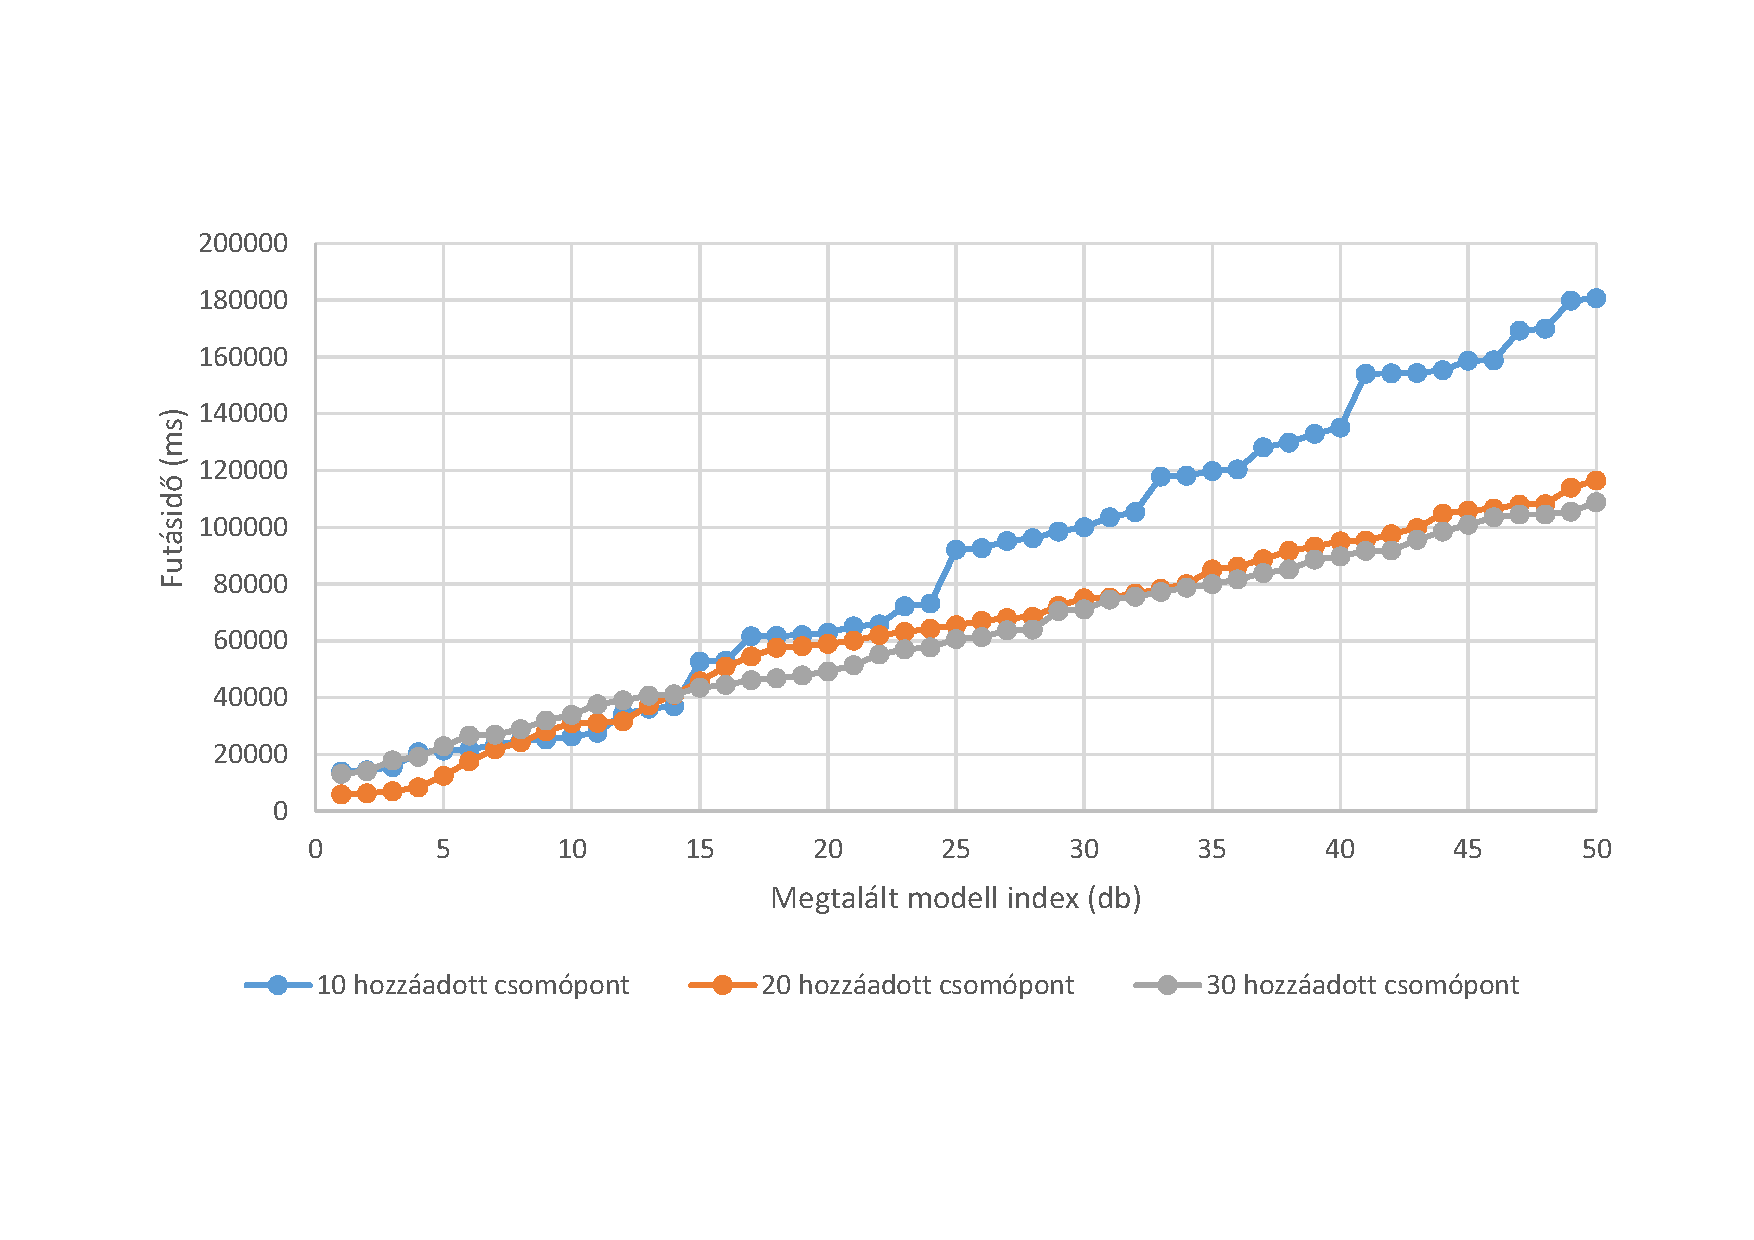
\includegraphics[width=1\textwidth]{figures/statisticsPlottalA}
	\caption{A K2 mérés eredményei}
	\label{fig:AmeresEredmeny}
\end{figure}
                                                                                                                                                                                                                                                                                           
A harmadik kérdésre az M1-es környezetben kerestem a választ. A mérés eredményei \aref{fig:AmeresEredmeny}. ábrán láthatóak. Az 50 darab generált modell megtalálásának ideje nem volt azonos a 10 alkalommal, ezért a 10 érték mediánját kiválasztottam, az ábrán ezeket a medián értékeket jelenítem meg. A 3 méret mérési eredményeit 3 színnel jelöltem. Az ábrán a függőleges tengelyen a futásidő látható milliszekundumban,  a vízszintes tengelyen pedig a létrejött tesztkészlet mérete.  

A három mérés eredményei lineárisak különböző meredekséggel, ez azt jelenti, hogy az egyes modellek megtalálása körülbelül ugyanannyi időt vesz igénybe. Ezen az ábrán is látható, hogy a generátor lassabban végzett a kis modellek megtalálásával mint a nagyokéval. 
                                                                                                               
\textit{Mivel közel lineáris egyenesek születtek a mérés eredményeként, levonható a következtetés, hogy az egyes modelleket körülbelül azonos időközönként találja meg a generátor,  tehát a modellek darabszámának függvényében remekül skálázódik a módszer.}

\section{Diverzitás mérése}


\begin{figure}[htp]
	\centering
	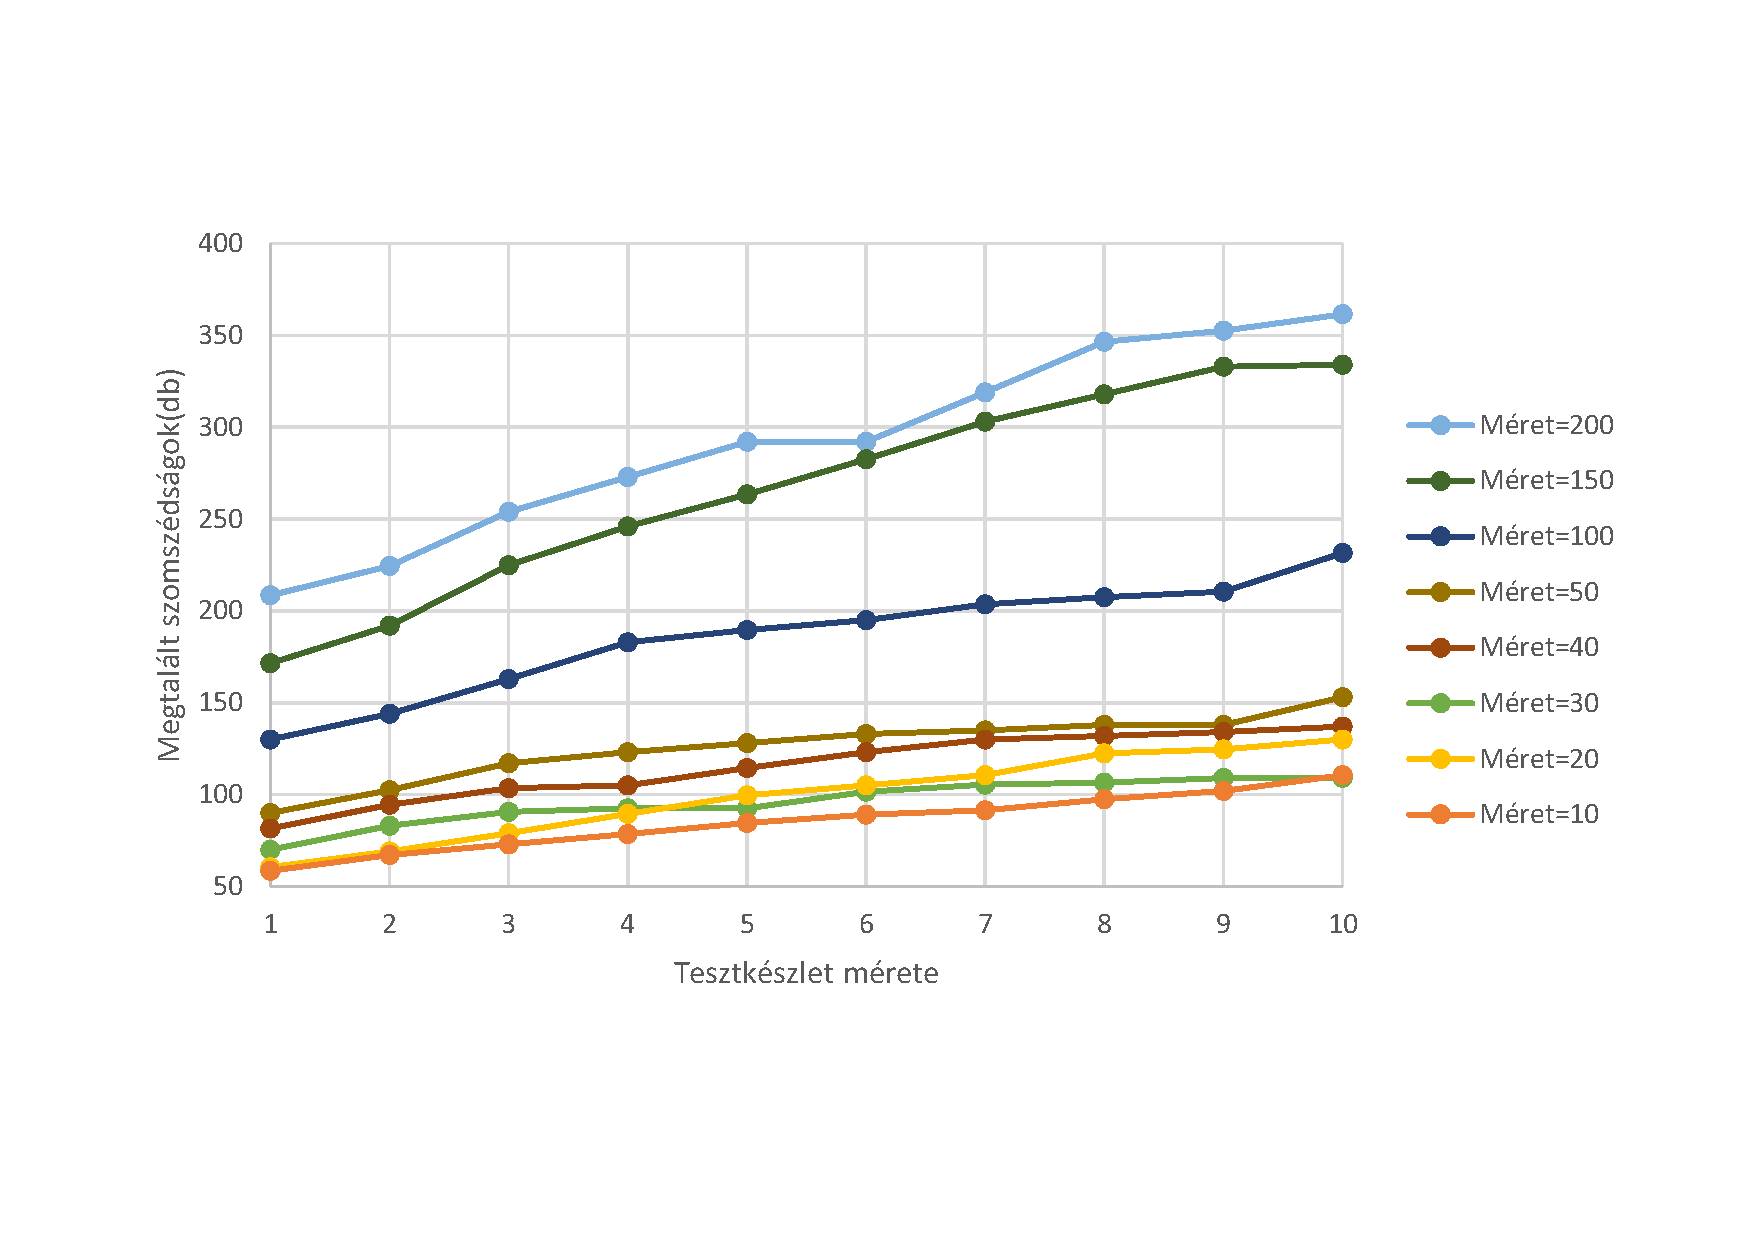
\includegraphics[width=1\textwidth]{figures/diversityB}
	\caption{A K2-es mérés diverzitása}
	\label{fig:BDiversity}
\end{figure}

Az M1 es környezetben végzett mérések során generált lekérdezések diverzitását is kimértem. Ezt szomszédsági formák segítségével tettem. A mérés eredményei \aref{fig:BDiversity}. ábrán láthatóak. Az ábra vízszintes tengelyén a tesztkészlet mérete látható, míg a függőleges tengelyen a megtalált szomszédságok darabszáma 3-as távolságban mérve. Az ábrázolt értékek a különböző minimális hozzáadott elemszámok esetén a 10 mérés mediánját mutatják.

Az ábrán látható, hogy a szomszédságok száma körülbelül lineárisan növekszik az különböző esetekben. A nagyobb lekérdezések esetén azért sokkal több a szomszédság mint a kisebbek esetén, mert ezen az ábrán már a Cypher nyelvre lefordított, nevekkel kitöltött lekérdezések szomszédságait ábrázoltam.

\textit{Levonható tehát a következtetés, hogy a diverzitás kezdetben folyamatosan közel lineárisan növekszik és nagyobb modellek esetén mindig nagyobb diverzitást érünk el.}  

\begin{figure}[htp]
	\centering
	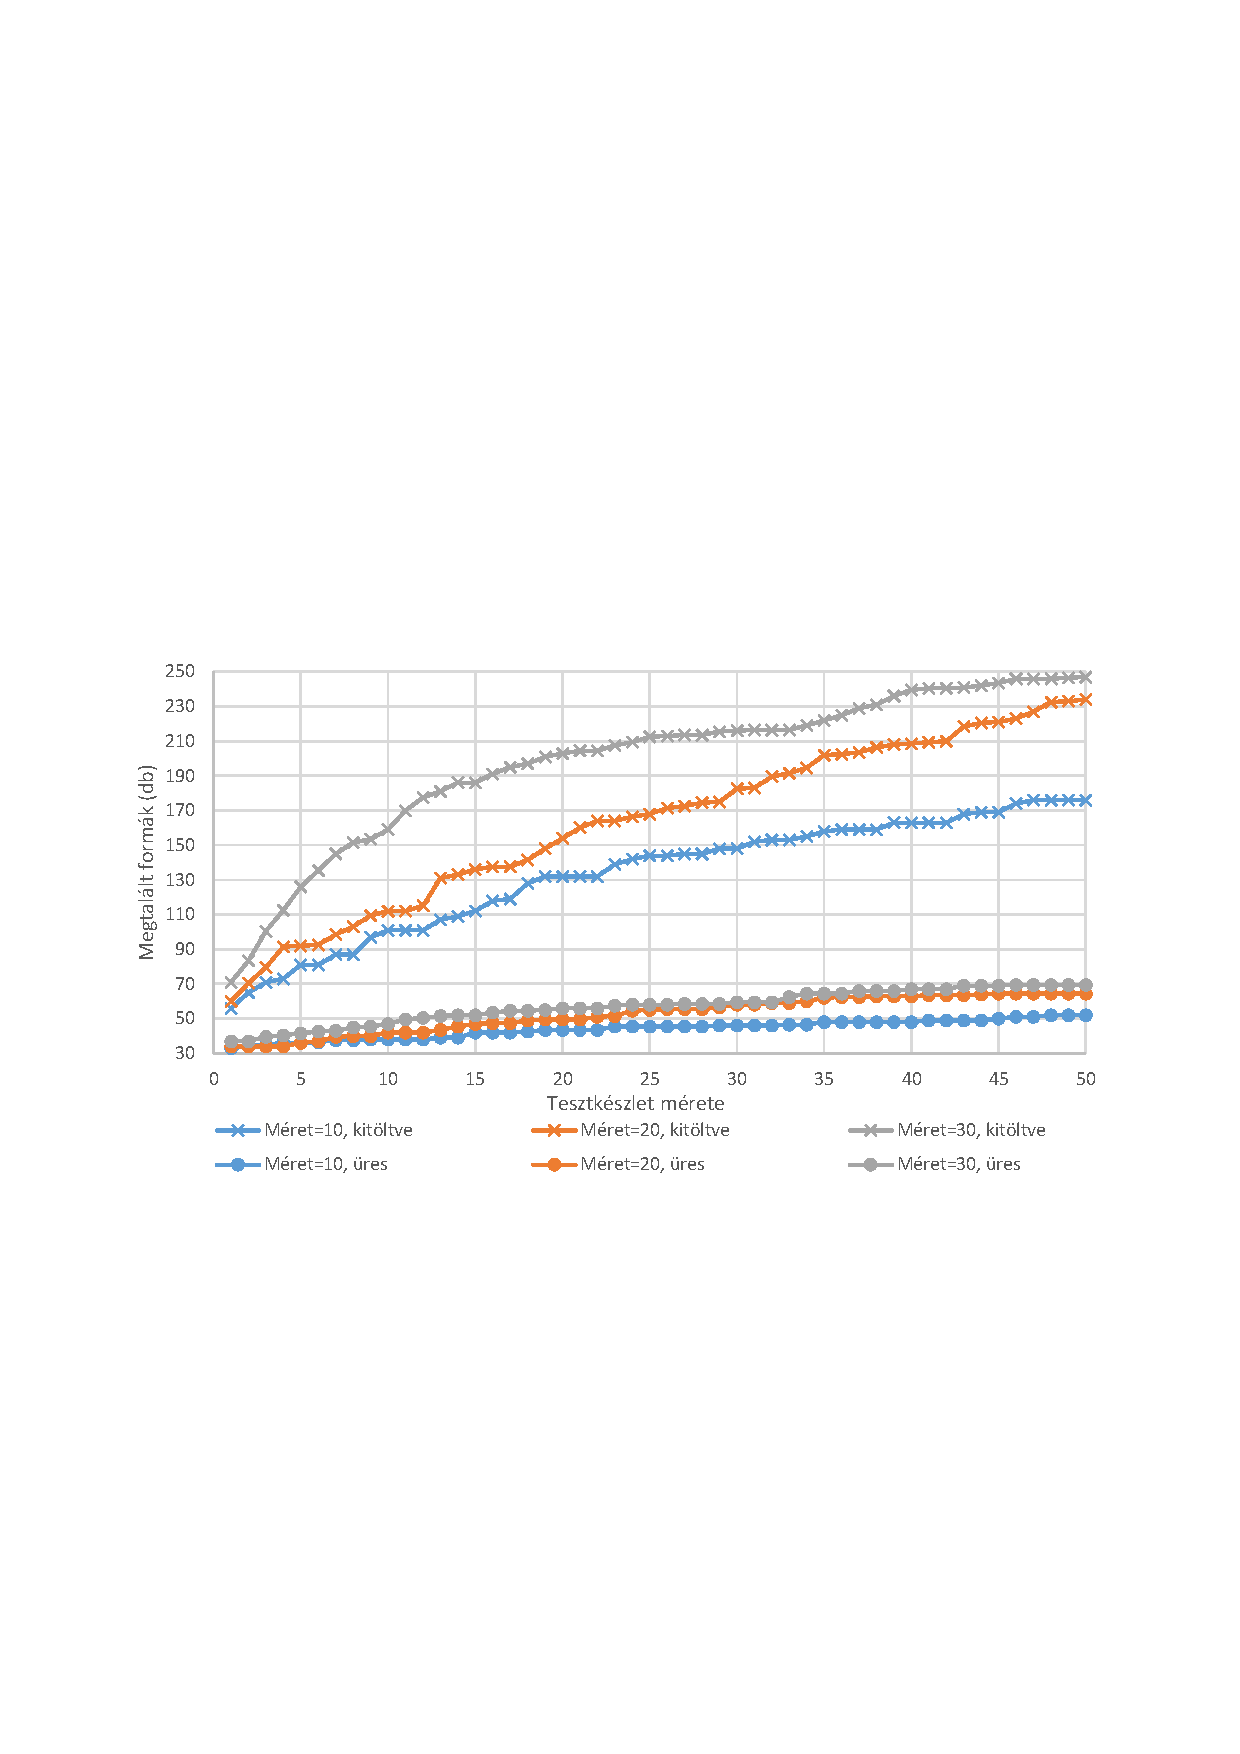
\includegraphics[width=1\textwidth]{figures/diversityA}
	\caption{K3-as mérés diverzitása}
	\label{fig:ADiversity}
\end{figure}

Az M2-es környezetben a lekérdezések és nyers kitöltetlen gráfok diverzitását egyaránt kimértem. A mérés eredményei
\aref{fig:ADiversity}. ábrán láthatóak. Az ábra vízszintes tengelyén a tesztkészlet mérete látható,  a függőleges tengelyen pedig a megtalált szomszédságok darabszáma. Az ábrázolt értékek a 10 elvégzett mérés során kapott értékek mediánjai. 

Az ábrán látható, hogy a kitöltetlen modellek sokkal kisebb diverzitást mutatnak mint a kitöltöttek. Illetve az is látható, hogy a kevés modellnél még lineárissal közelíthető növekedés sok modellnél logaritmikussá alakul. 

\textit{Az általam bevitt diverzitás növelését segítő módszerek tehát hatékonyak, illetve a generálás során a diverzitás folyamatosan növekszik.}

\section{Lekérdezések futásidejének mérése Neo4j adatbázison}

\begin{figure}[htp]
	\centering
	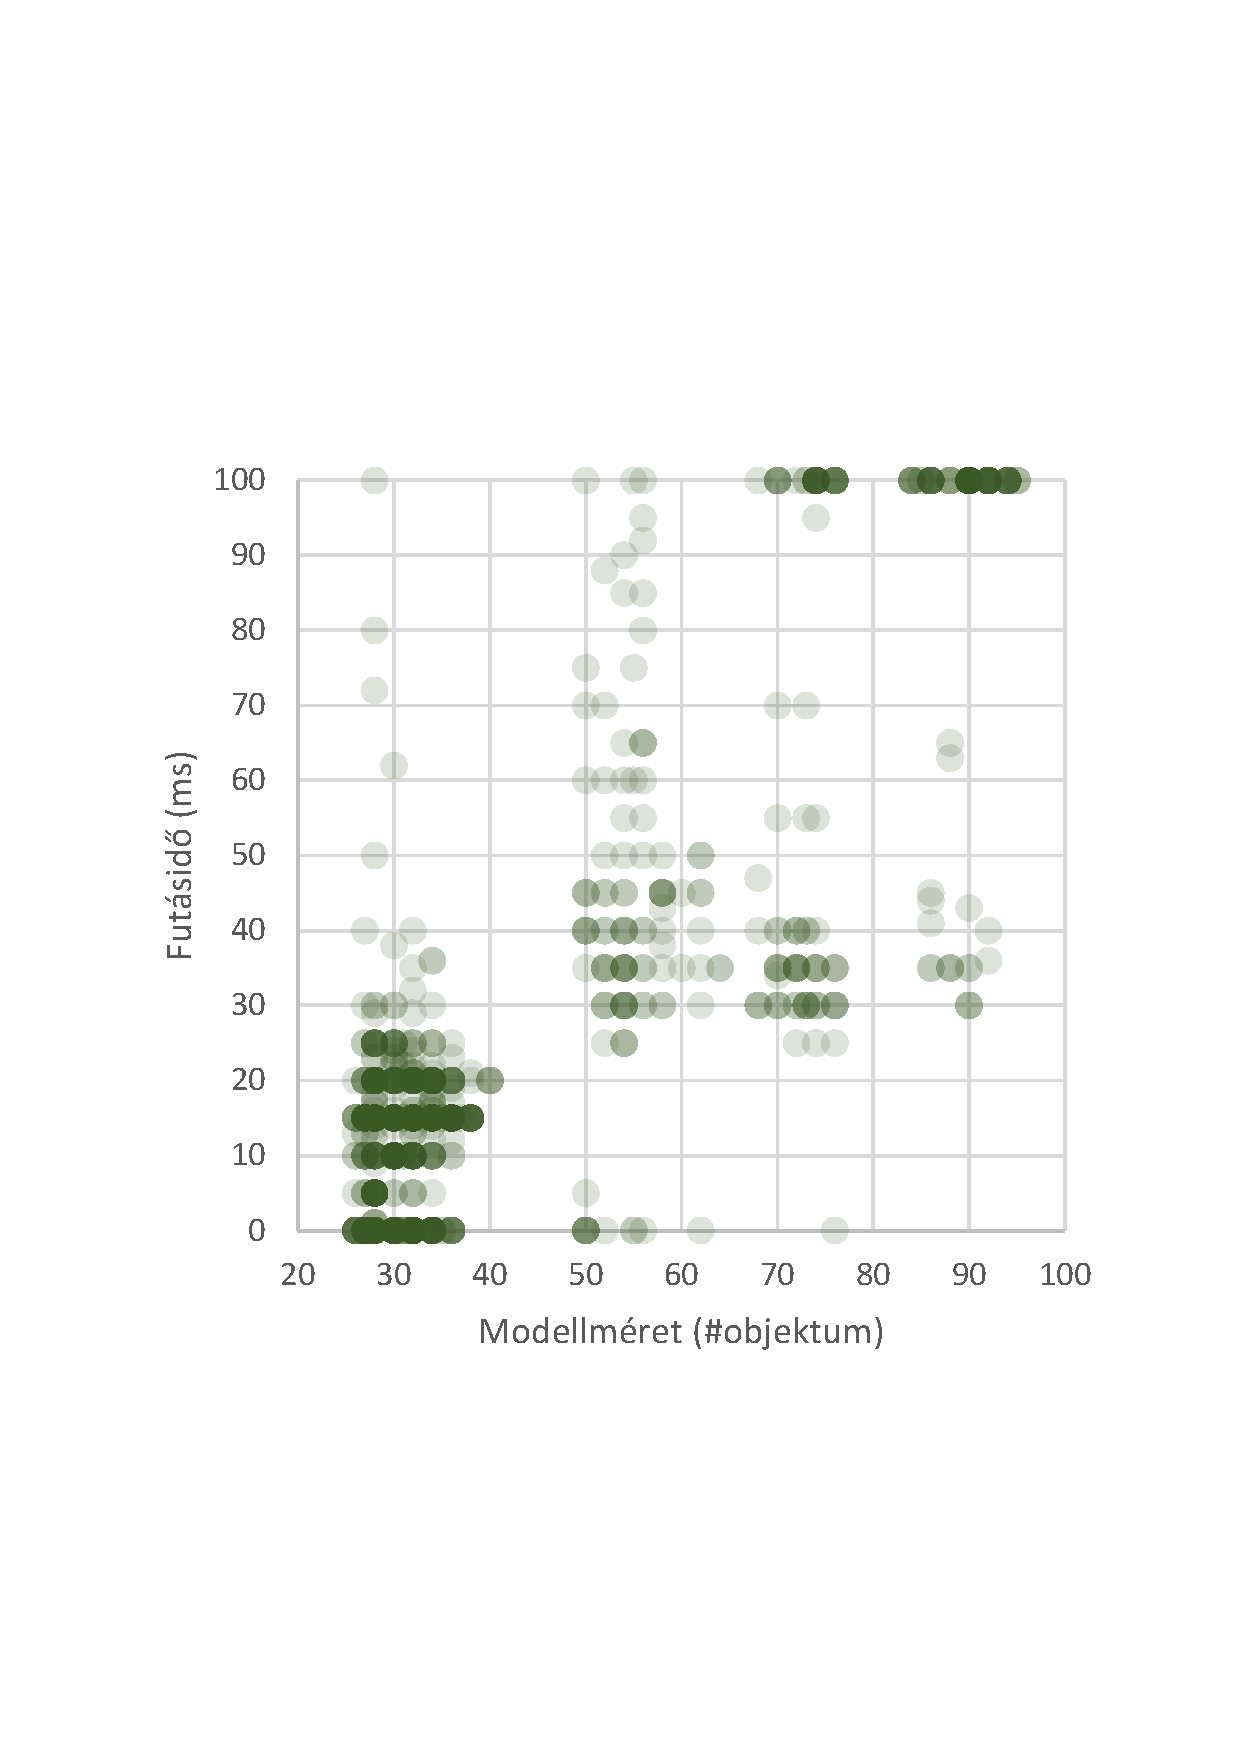
\includegraphics[width=0.6\textwidth]{figures/measurementRuntimeResultNeo4J}
	\caption{Lekérdezéseim futásidejének eredménye}
	\label{fig:Neo4jRuntime}
\end{figure}

Az M2-es környezetben generált lekérdezéseket egy a Train Benchmark által összeállított adatbázison futtattam, amelyben 2024 csomópont és ezek között 5878 kapcsolat volt.
A lekérdezéseket két állapotban futtattam le: (1) attribútumok meghagyásával, és (2) kiszűrésével.
 

Az első futás alkalmával az általam generált lekérdezésekben szereplő attribútum feltételek nem tettek eleget az adatbázisban szereplő attribútum értékeknek, így a legtöbb lekérdezés 0 ms-os eredménnyel nem futott le (ezt ábrán nem szemléltetem).

\textit{Ezzel a méréssel felfedeztük, hogy a Neo4j az attribútumok alapján indexel, és hatékonyan meg tudja válaszolni az ezekkel kapcsolatos lekérdezéseket.}

A második mérés eredményét \aref{fig:Neo4jRuntime}.~ábrán szemléltetem. A pontok az egyes modellekhez tartozó futásidőket jelenítik meg. A vízszintes tengelyen a modellek mérete látható, az alapján számolva hogy hány csomópontból áll az ASG-jük, a függőleges tengelyen pedig a hozzájuk tartozó futásidő. A sötétebb pontok azt jelentik, hogy ott sok egyforma érték született, a halványabbaknál kevesebb. A futásidőt 100-ban maximalizáltam. 

Az ábrán látható, hogy a kisebb modellek kisebb, a közepesek közepes, a nagyok pedig nagyon nagy futásidőt mutatnak, az is látható, hogy míg a kisebb modelleknél volt kevés olyan lekérdezés ami nagyon lassan futott le, addig a nagyobbaknál nem volt olyan ami nagyon gyorsan futott volna le.

 
\textit{Következtetésként levonhatjuk, hogy a generált modellek mérete és a futásidő gyengén korrelál.}

\section{Lehetséges mérési hibák}
\begin{itemize}
	\item Egyetlen esettanulmányon futtattam a méréseket, de ez egy reprezentatív, korszerű, aktívan fejlesztett teljesítmény benchmark, amelyet már több más esettanulmányban is alkalmaztak.\cite{garcia2017stress, bur2018distributed} 
	\item Csak pozitív mintájú lekérdezések generálásával foglalkoztam. Mivel ezek adják az összes lekérdezés alapját a tőlem függetlenül fejlesztett nyelvtanban, jó reprezentatív esetnek számítanak. 
	\item A mérések során mindent csak 10-szer futtattam, de a futásidők és a diverzitások nem mutattak nagy eltéréseket egymástól. A mérési zajt medián számítással mértem ki. A bemelegedés hatását pedig bemelegítő mérések hozzáadásával küszöböltem ki az éles mérések előtt, megvárva a futásidő stabilizálódását.
	\item Bár korrelációt mutat a futásidő és a lekérdezés bonyolultsága ebből egyelőre komolyabb következtetést nem vonhatunk le, ennek értékelése további vizsgálatokat kíván. 	
\end{itemize}





\chapter{Kapcsolódó munkák}
\label{chp:6}

Az alábbiakban összefoglalom, a munkámhoz kapcsolódó szakirodalmat. A modellgenerálás fejezet ennek \cite{semerath2018iterative} a cikknek a felépítését követi.  

\section{Modell és gráfgenerálás}

A diverz modell generálás kulcsfontosságú szerepet játszik modell transzformációk, kód generátorok és komplett fejlesztőrendszerek tesztelése során. A mutáció alapú megközelítések \cite{aranega2015towards}, \cite{darabos2008towards}  létező modelleken hajtanak végre véletlenszerű változtatásokat mutációs szabályok alkalmazásával. Más automatizált technikák  \cite{brottier2006metamodel}, \cite{ehrig2009generating}, olyan modelleket generálnak, amelyek csak a metamodellhez alkalmazkodnak. Míg ez  az utóbbi megoldás jól skálázódik nagyobb modellekre, addig a mutációs módszerrel generált modelleknél nincs arra  garancia, hogy jólformáltak lesznek.

A modellgeneráló technikák egy nagyobb halmaza bizonyos ígéreteket ad a teszt hatékonyságára. Az ilyen white-box alapú megközelítések \cite{aranega2015towards}, \cite{bordbar2005uml2alloy} implementáción és transzformáción alapulnak, és általában back-end logikai megoldókat használnak, amelyek nem jól skálázhatóak gráfmodellekre.

A black-box megközelítések \cite{buttner2012verification}, \cite{fleurey2007towards}, csak a specifikációját használják fel a nyelvnek, vagy a transzformációnak, így alapvetően  kényszereken, illetve részmodelleken alapulnak. Ezekben a megközelítésekben közös, hogy néha egyszerű modelleket generálnak, amelyeknek   növelhető ugyan diverzitása szimmertia-törő predikátumokkal, de nagyobb modellekre nem skálázódnak. Sőt,  a modellek effektív diverzitása is megkérdőjelezhető, mert a jelenlegi modell- transzformációkat tesztelő módszerekben sokkal enyhébb vizsgálatoknak kell csak megfelelni, mint a különböző szoftverek tesztelése során.

\section{Adatbázis tesztelés}

Az adatbázisok tesztelése egy nehéz, aktívan kutatott feladat, amelynek több hasonló megközelítése is megtalálható a szakirodalomban.


Az enyémhez leghasonlóbb megközelítés a \cite{DBLP:conf} cikkben leírt ADUSA keretrendszer, ami szintén SAT alapú megoldókkal dolgozik, ők Alloy-t \cite{Alloy:Language} , \cite{alloy:kodkod} használnak. Az ő módszerük az enyémmel ellentétben SQL specifikus és nyelv alapján úgy tűnik hogy csak fix méretű modellek generálására alkalmas. A \textsc{Viatra} Solver is támogatja az Alloy-t mint mögöttes megoldót Cypher lekérdezések generálására viszont azt tapasztaltam, hogy nem skálázódik megfelelően. Másrészt korábbi tapasztalatok alapján \cite{semerath2018iterative} gyenge minőségű tesztkészletet állít elő diverzitás szempontjából.


Az \cite{myint2018test} cikk a páronkénti fedettség (pairwise testing) tesztelési módszert javasolja adatbázisok tesztelésére. Ez azt jelenti, hogy első lépésben részekre bont egy lekérdezést, majd a másodikban minden részletre felsorol lehetséges részkifejezéseket, majd ezekből a részkifejezésekből készít helyes lekérdezéseket úgy, hogy minden lehetséges részletpár legalább egyszer szerepeljen. (Anélkül, hogy explicit az összes kombinációt elő kelljen állítani.) Ehhez képest a megközelítésem során nem szükséges explicit felsorolni lekérdezés részleteket, hanem ezeket automatikusan állítom elő. Továbbá az általam biztosított fedettség hasonló a  páronkénti fedettséghez, hiszen a generálás során az összes különböző szomszédságú gráfcsomópont felfedezését biztosítjuk.
	 
 Az \cite{yan2018snowtrail} cikkben egy felhő alapú adatbázisban végeznek regressziós tesztelést, az enyémhez hasonló felépítés segítségével, csak itt a teszt lekérdezések halmazát a felhasználók által korábban írt és futtatott lekérdezésekből válogatják össze így próbálva biztosítani a diverzitást. Ezzel szemben én automatikusan generálok lekérdezéseket, ami ezáltal remekül egészíti ki ezt a megközelítést olyan esetben, amikor a lekérdezések nem hozzáférhetőek. 

A \cite{tuya2006sqlmutation} cikkben alkalmazott módszer során relációs adatbázisok teszteléséhez generálnak SQL lekérdezéseket mutációs módszerrel. Ennek a megközelítésnek több hátránya is van amit az én megközelítésem kiküszöböl. Egyrészt szükség van egy nagyobb meglévő tesztkészletre, másrészt a mutánsok hasonlítanak az eredeti teszt készletre ezért rossz minőségű tesztkészletet alkotnak diverzitás szempontjából. 

A \cite{SuarezCabal} cikkben SQL specifikus struktúrális metrikákat javasolnak a nagyobb tesztfedettség eléréséhez. Én is ehhez hasonlóakat használok általánosan.

A \cite{DBLP} cikkben a módszeremmel ellentétben white-box alapú adatbázis tesztelési módszert javasolnak, mégpedig úgy, hogy a lekérdezéseket végrehajtható forráskóddá alakítják és így tesztorákulumot képeznek.



\section{Adatbázis benchmarkolás}
Sok adatbázis benchmark létezik, egy válogatást a \cite{szarnyas2018train} cikkből emeltem ki az alábbi táblázatba. A táblázat alsó sorában az látható, hogy a benchmarkolásra hány lekérdezést használtak fel. Ezzel szemben munkám során én megközelítőleg 3000 lekérdezést generáltam. Az eddigi benchmarkoklási technikák fő hiányosságának a lekérdezések mennyisége tűnik.  Ezáltal a megközelítésem alkalmazásával forradalmasítani lehetne az adatbázisok teljesítmény tesztelését. 

\begin{center}
	\begin{tabular}{ c | c | c | c | c | c | c }
 LUBM & Barton & SP2Bench & 	BSBM & DBpedia & LDBC SNB &	Train Benchmark \\\hline
 14 & 7 & 12 & 12 &	25 & 14 & 	6 \\
	\end{tabular}
\end{center}

\noindent
Tudomásom szerint nincs olyan adatbázis benchmark ami szintetikus lekérdezéseket futtat.
\chapter{Összefoglaló és jövőbeli munkák}
\label{chp:7}

A dolgozatomban sikerrel megvalósítottam egy többlépéses gráflekérdezés generálási folyamatot, amely képes volt Neo4j adatbázis által beolvasható és feldolgozható lekérdezéseket előállítására. A generátor paraméterezhető a vizsgálni kívánt adatbázis tartalmával (címkekészlet), valamint a lekérdezések mennyiségével és bonyolultságával.
Ezen felül biztosítja lekérdezések diverzitását, így minden kiadott lekérdezés különbözik a többitől.
Az általam készített keretrendszert teljesítmény és diverzitás szempontjából is kiértékeltem egy ipari esettanulmányon, valamint korrelációt is találtunk a lekérdezések bonyolultsága és futásideje között.
Továbbá kiemelendő, hogy dolgozatomban számos technológiát alkalmaztam:
 \begin{itemize}
 	\item Gráfadatbázisok területén: Cypher gráfadatbázisnyelv, Neo4j adatbázis, Train Benchmark esettanulmány.
 	\item Modellezés területén: Eclipse Modeling Framework modellező keretrendszer, Xtext technológia lekérdezések beolvasáshoz és sorosításhoz (konkrétan a slizaa nyelvtant használva), \textsc{Viatra} gráfmintaillesztő rendszer jólformáltsági kényszerek meghatározására, és Xtend-et modellek utófeldolgozására.
 	\item Matematikai eszközök:\textsc{Viatra} Solver gráfgeneráláshoz, illetve a prototipizáláshoz Alloy gráfgenerátor Sat4j mögöttes SAT megoldóval (amely skálázódási okok miatt nem volt alkalmas komolyabb mérések elvégzéséhez).
 	Elméleti eredményként elmondható, hogy sikerrel alkalmaztam egy fejlett gráfgenerálási algoritmust
 \end{itemize}

Elméleti eredményként elmondható, hogy Cypher nyelv slizaa nyelvtanának nyelvtani szabályait absztrakt szintaxis gráfon értelmezhető gráfmintákként formalizáltam \textsc{Viatra} nyelven. Ezáltal a nyelv feldolgozhatóvá vált logikai következtetőkkel, amit sikerrel alkalmaztam lekérdezések szintetizálásához. Ezen felül a Cypher nyelv szimmetrikus megfogalmazásait modell-szimmetriaként fogalmaztam meg, így javítva a lekérdezések diverzitását.

Sikerként mondható el, hogy már sikerült is találni szemantikus eltérést a tanszékemen fejlesztett InGraph 
\cite{MartonSB17} és a referenciaimplementáció Neo4j rendszerekben. Ezen kívül felkerestük a Neo4j fejlesztőit is, akiknek felkeltette az érdeklődését a fejlesztett eszköz.

Jövőbeli munkaként az általam készített lekérdezés generátor kiegészíthető lehet olyan komplex gráfadatbázis-tartalmak előállításával, mellyel az így előálló rendszer akár egy komplett környezetet biztosíthatna gráfadatbázisok tesztelésére és teljesítménymérésére, előállítva a teljes bemenetet.





% Acknowledgements
%~~~~~~~~~~~~~~~~~~~~~~~~~~~~~~~~~~~~~~~~~~~~~~~~~~~~~~~~~~~~~~~~~~~~~~~~~~~~~~~~~~~~~~
%%----------------------------------------------------------------------------
\chapter*{\koszonetnyilvanitas}\addcontentsline{toc}{chapter}{\koszonetnyilvanitas}
%----------------------------------------------------------------------------

Ez nem kötelező, akár törölhető is. Ha a szerző szükségét érzi, itt lehet köszönetet nyilvánítani azoknak, akik hozzájárultak munkájukkal ahhoz, hogy a hallgató a szakdolgozatban vagy diplomamunkában leírt feladatokat sikeresen elvégezze. A konzulensnek való köszönetnyilvánítás sem kötelező, a konzulensnek hivatalosan is dolga, hogy a hallgatót konzultálja.


% List of Figures, Tables
%~~~~~~~~~~~~~~~~~~~~~~~~~~~~~~~~~~~~~~~~~~~~~~~~~~~~~~~~~~~~~~~~~~~~~~~~~~~~~~~~~~~~~~
%\listoffigures\addcontentsline{toc}{chapter}{\listfigurename}
%\listoftables\addcontentsline{toc}{chapter}{\listtablename}


% Bibliography
%~~~~~~~~~~~~~~~~~~~~~~~~~~~~~~~~~~~~~~~~~~~~~~~~~~~~~~~~~~~~~~~~~~~~~~~~~~~~~~~~~~~~~~
\addcontentsline{toc}{chapter}{\bibname}
\bibliography{bib/mybib}


% Appendix
%~~~~~~~~~~~~~~~~~~~~~~~~~~~~~~~~~~~~~~~~~~~~~~~~~~~~~~~~~~~~~~~~~~~~~~~~~~~~~~~~~~~~~~
%%----------------------------------------------------------------------------
\appendix
%----------------------------------------------------------------------------
\chapter*{\fuggelek}\addcontentsline{toc}{chapter}{\fuggelek}
\setcounter{chapter}{\appendixnumber}
%\setcounter{equation}{0} % a fofejezet-szamlalo az angol ABC 6. betuje (F) lesz
\numberwithin{equation}{section}
\numberwithin{figure}{section}
\numberwithin{lstlisting}{section}
%\numberwithin{tabular}{section}

%----------------------------------------------------------------------------
\section{A TeXstudio felülete}
%----------------------------------------------------------------------------
\begin{figure}[!ht]
\centering
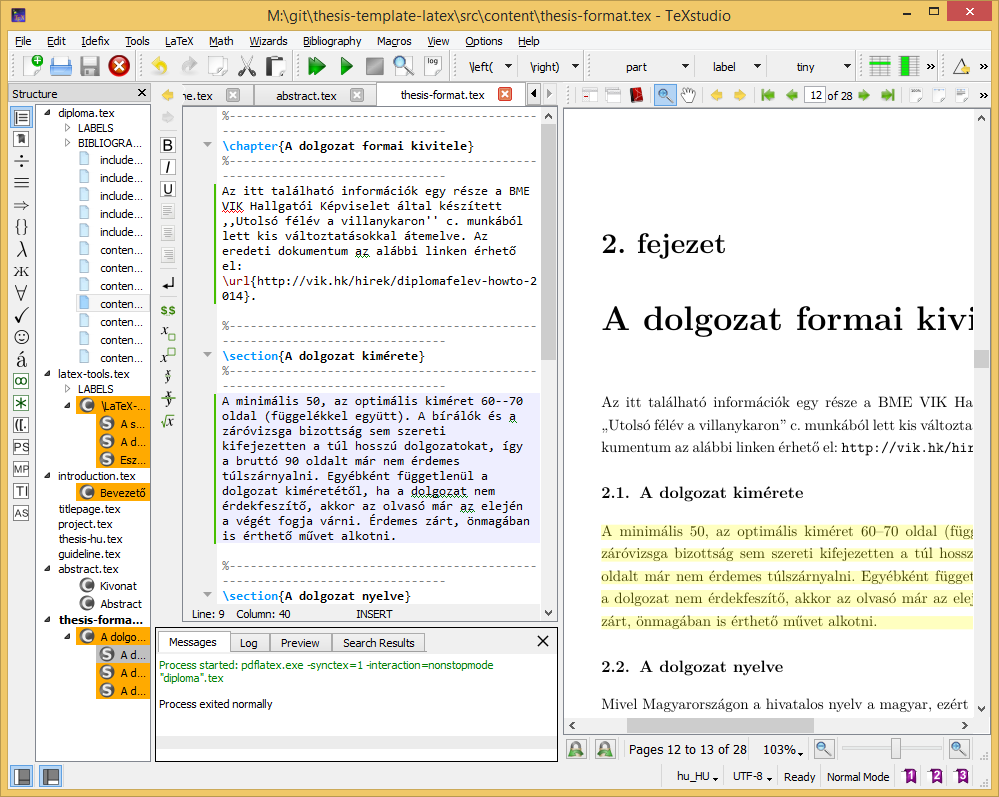
\includegraphics[width=150mm, keepaspectratio]{figures/TeXstudio.png}
\caption{A TeXstudio \LaTeX-szerkesztő.} 
\end{figure}

%----------------------------------------------------------------------------
\clearpage\section{Válasz az ,,Élet, a világmindenség, meg minden'' kérdésére}
%----------------------------------------------------------------------------
A Pitagorasz-tételből levezetve
\begin{align}
c^2=a^2+b^2=42.
\end{align}
A Faraday-indukciós törvényből levezetve
\begin{align}
\rot E=-\frac{dB}{dt}\hspace{1cm}\longrightarrow \hspace{1cm}
U_i=\oint\limits_\mathbf{L}{\mathbf{E}\mathbf{dl}}=-\frac{d}{dt}\int\limits_A{\mathbf{B}\mathbf{da}}=42.
\end{align}


%\label{page:last}
\end{document}
